\documentclass[12pt]{report} 
  \usepackage{threeparttable}
  \usepackage{geometry}
  \geometry{letterpaper,tmargin=1in,bmargin=1in,lmargin=1.25in,rmargin=1.25in}
  \usepackage[format=hang,font=normalsize,labelfont=bf]{caption}
  \usepackage{amsmath}
  \usepackage{multirow}
  \usepackage{array}
  \usepackage{delarray}
  \usepackage{amssymb}
  \usepackage{amsthm}
  \usepackage{lscape}
  \usepackage{natbib}
  \usepackage{setspace}
  \usepackage{float,color}
  \usepackage[pdftex]{graphicx}
  \usepackage{pdfsync}
  \usepackage{verbatim}
  \usepackage{placeins}
  \synctex=1
  \usepackage{hyperref}
  \hypersetup{colorlinks,linkcolor=red,urlcolor=blue,citecolor=red}
  \usepackage{bm}
  \usepackage{makeidx}       % Package to make an index.

  \theoremstyle{definition}
  \newtheorem{theorem}{Theorem}
  \newtheorem{acknowledgement}[theorem]{Acknowledgement}
  \newtheorem{algorithm}[theorem]{Algorithm}
  \newtheorem{axiom}[theorem]{Axiom}
  \newtheorem{case}[theorem]{Case}
  \newtheorem{claim}[theorem]{Claim}
  \newtheorem{conclusion}[theorem]{Conclusion}
  \newtheorem{condition}[theorem]{Condition}
  \newtheorem{conjecture}[theorem]{Conjecture}
  \newtheorem{corollary}[theorem]{Corollary}
  \newtheorem{criterion}[theorem]{Criterion}
  \newtheorem{definition}{Definition} % Number definitions on their own
  \newtheorem{derivation}{Derivation} % Number derivations on their own
  \newtheorem{example}[theorem]{Example}
  \newtheorem{exercise}[theorem]{Exercise}
  \newtheorem{lemma}[theorem]{Lemma}
  \newtheorem{notation}[theorem]{Notation}
  \newtheorem{problem}[theorem]{Problem}
  \newtheorem{proposition}{Proposition} % Number propositions on their own
  \newtheorem{remark}[theorem]{Remark}
  \newtheorem{solution}[theorem]{Solution}
  \newtheorem{summary}[theorem]{Summary}
  \bibliographystyle{aer}
  \newcommand\ve{\varepsilon}
  \newcommand{\cn}{\citeasnoun} % shortens command to cite as noun
  \renewcommand\theenumi{\roman{enumi}}
  \newcommand\norm[1]{\left\lVert#1\right\rVert}
  
  \makeindex    % Make the index

\begin{document}

%titlepage
\begin{titlepage}
  \title{Dyanmic General Equilibrim Tax Scoring Model
    \thanks{We are grateful to Kevin Hassett, Alan Viard, Alex Brill, Matt Jensen, Aspen Gorry, Frank Caliendo, and Richard W. Evans, Sr. for helpful comments and suggestions. This research benefited from support from Brigham Young University Macroeconomics and Computational Laboratory and the Open Source Policy Center at the American Enterprise Institute. All Python code for the computational model is available at \href{https://github.com/OpenSourcePolicyCenter/dynamic}{https://github.com/OpenSourcePolicyCenter/dynamic}.} }

  \author{
  Jason DeBacker\footnote{Middle Tennessee State University, Department of Economics and Finance, BAS N306, Murfreesboro, TN 37132, (615) 898-2528,\href{mailto:jason.debacker@mtsu.edu}{jason.debacker@mtsu.edu}.} \\[-2pt]
  \and
  Richard W. Evans\footnote{Brigham Young University, Department of Economics, 167 FOB, Provo, Utah 84602, (801) 422-8303, \href{mailto:revans@byu.edu}{revans@byu.edu}.} \\[-2pt]
  \and
  Evan Magnusson\footnote{Brigham Young University, Department of Economics, 163 FOB, Provo, Utah 84602, \href{mailto:evanmag42@gmail.com}{evanmag42@gmail.com}.} \\[-2pt]
  \and
  Kerk L. Phillips\footnote{Brigham Young University, Department of Economics, 166 FOB, Provo, Utah 84602, (801) 422-5928, \href{mailto:kerk_phillips@byu.edu}{kerk\_phillips@byu.edu}.} \\[-2pt]
  \and
  Isaac Swift\footnote{Brigham Young University, Department of Economics, 163 FOB, Provo, Utah 84602, \href{mailto:isaacdswift@gmail.com}{isaacdswift@gmail.com}.} \\[-2pt]}
  \date{February 2015 \\
  \scriptsize{(version 15.02.a)}}
  \maketitle
  \begin{abstract}
  \small{An open source dynamic scoring model for U.S. federal tax policy...

  \vspace{0.3in}

  \textit{keywords:} dynamic general equilibrium, taxation, numerical simulation, computational techniques, simulation modeling.

  \vspace{0.3in}

  \textit{JEL classifications:} C63, C68, E62, H24, H25, H68}
  \end{abstract}
  \thispagestyle{empty}
\end{titlepage}

%%% 
% Table of Contents and Lists of Tables and Figures %
%%%

\tableofcontents   % Table of Contents will be automatically
                   % generated and placed here.
\listoftables      % List of Tables and List of Figures will be placed
\listoffigures     % here, if applicable.


%%% 
% Including files for different sections of handbook %
%%%
\chapter{Households}
\index{Households%
@\emph{Households}}%

  \section{Demographics}
    A measure $\omega_{1,t}$ of individuals with heterogeneous working ability $e \in\mathcal{E}\subset\mathbb{R}_{++}$ is born in each period $t$ and live for $E+S$ periods, with $S\geq 4$.\footnote{Theoretically, the model exposition of the model works without loss of generality for $S\geq 3$. However, because we are calibrating the ages outside of the economy to be one-fourth of $S$ (e.g., ages 21 to 100 in the economy, and ages 1 to 20 outside of the economy), we need $S$ to be at least 4.} The population of age-$s$ individuals in any period $t$ is $\omega_{s,t}$. Households are termed ``youth'', and do not participate in market activity, during ages $1\leq s\leq E$. The households enter the workforce and economy in period $E+1$ and remain in the workforce until they unexpectedly die or live until age $s=E+S$.\footnote{We model the population with households age $s\leq E$ outside of the workforce and economy in order most closely match the empirical population dynamics.} The population of agents of each age in each period, $\omega_{s,t}$, evolves according to the following function,
    \begin{equation}\label{EqPopLawofmotion}
      \begin{split}
        \omega_{1,t+1} &= \sum_{s=1}^{E+S} f_s\omega_{s,t}\quad\forall t \\
        \omega_{s+1,t+1} &= (1 + i_s - \rho_s)\omega_{s,t}\quad\forall t\quad\text{and}\quad 1\leq s \leq E+S-1
      \end{split}
    \end{equation}
    where $f_s\geq 0$ is an age-specific fertility rate, $i_s$ is an age-specific immigration rate, $\rho_s$ is an age specific mortality hazard rate,\footnote{The parameter $\rho_s$ is the probability that a household of age $s$ dies before age $s+1$.} and $1+i_s-\rho_s$ is constrained to be nonnegative. The total population in the economy $N_t$ at any period is simply the sum of individuals in the economy, the population growth rate in any period $t$ from the previous period $t-1$ is $g_{n,t}$, $\tilde{N}_t$ is the working age population, and $\tilde{g}_{n,t}$ is the working age population growth rate in any period $t$ from the previous period $t-1$.
    \begin{equation}\label{EqPopDef}
      N_t\equiv\sum_{s=1}^{E+S} \omega_{s,t} \quad\forall t
    \end{equation}
    \begin{equation}\label{EqPopGrowth}
      g_{n,t+1} \equiv \frac{N_{t+1}}{N_t} - 1 \quad\forall t
    \end{equation}
    \begin{equation}\label{EqPopWkDef}
      \tilde{N}_t\equiv\sum_{s=E+1}^{E+S} \omega_{s,t} \quad\forall t
    \end{equation}
    \begin{equation}\label{EqPopWkGrowth}
      \tilde{g}_{n,t+1} \equiv \frac{\tilde{N}_{t+1}}{\tilde{N}_t} - 1 \quad\forall t
    \end{equation}


  \section{Households}
  Consumer's are forward-looking, intertemporal optimizers.  Their objective is the maximize the expected, discounted value of lifetime utility.  Expectations are taken over mortality risk, the only source of uncertainty in the model.  Individuals are heterogenous with repeat to age and lifetime income group.  We define the expected, discounted lifetime utility at time $t$ for an individual in lifetime income group $j$ and age $s$ to be $U_{j,s,t}$.  We assume that utility is additively separable across periods and thus write expected, discounted lifetime utility as:
    \begin{equation}\label{EqUtilMax}
      \begin{split}
        &U_{j,s,t} = \sum_{u=0}^{E+S-s}\beta^u\left[\prod_{v=s-1}^{s+u-1}(1-\rho_v)\right] u\left(c_{j,s+u,t+u},n_{j,s+u,t+u},b_{j,s+u+1,t+u+1}\right) \\
        &\text{where}\quad \rho_{s-1}=0 \\
        &\text{and} \quad u\left(c_{j,s,t},n_{j,s,t},b_{j,s+1,t+1}\right) = \frac{\left(c_{j,s,t}\right)^{1-\sigma} - 1}{1-\sigma} ... \\
        &\qquad\qquad + e^{g_y t(1-\sigma)}\chi^n_s\left(b\left[1 - \left(\frac{n_{j,s,t}}{\tilde{l}}\right)^\upsilon\right]^\frac{1}{\upsilon} + k\right) + \rho_s\chi^b\frac{\left(b_{j,s+1,t+1}\right)^{1-\sigma} - 1}{1-\sigma} \\
        &\quad\quad\quad\quad\quad\quad\quad\quad\quad\quad\quad\quad\quad\quad\quad\quad\quad\quad\quad\forall j,t\quad\text{and}\:E+1\leq s\leq E+S
      \end{split}
    \end{equation}

\noindent\noindent The parameter $\beta\in(0,1)$ represents the individual's rate of time preference.  The quantities $c_{j,s,t}$, $n_{j,s,t},$ and $b_{j,s,t}$ are total consumption of a composite consumption good, labor supply, and asset holdings, respectively.  The parameter $\sigma \geq 1$ is the coefficient of relative risk aversion, $\upsilon$ is a measure of the elasticity of labor supply, and $\tilde{l}$ is the total time endowment of the individual.  The utility weight for the disutility of labor is given by the age-dependent parameters $\chi^{n}_{s}$.  The parameter $g_y$ is a constant growth rate of labor augmenting technological progress, which we explain in more detail in the firm's problem .\footnote{The term with the growth rate $e^{g_y t(1-\sigma)}$ must be included in the period utility function because consumption and bequests will be growing at rate $g_y$ and this term stationarizes the individual Euler equation by making the marginal disutility of labor grow at the same rate as the marginal benefits of consumption and bequests.  This is the same balanced growth technique as that used in \citet{MertensRavn:2011}.}  The disutility of labor term in the utility function looks nonstandard, but is simply the upper quadrant of an ellipse that closely approximates the standard constant relative risk aversion utility of leisure functional form.\footnote{Appendix \ref{AppEllipseUtil} describes how the elliptical function closely matches the more standard utility of leisure of the form $\frac{(\tilde{l}-n_{j,s,t})^{1-\eta} - 1}{1-\eta}$. The parameters $b$ and $k$ are the scale and shift parameters of describing the elliptical form.  This elliptical utility function forces an interior solution that automatically respects both the upper and lower bound of labor supply, which greatly simplifies the computation of equilibrium.  For a more in-depth discussion see \citet{EvanPhillips:2015}} The utility weight on bequests (both intentional and accidental) is given by $\chi^{b}$.

 \begin{figure}[htb]\centering \captionsetup{width=4.0in}
\caption{\label{fig:hh_tree}\textbf{Summary of the Individual Problem}}
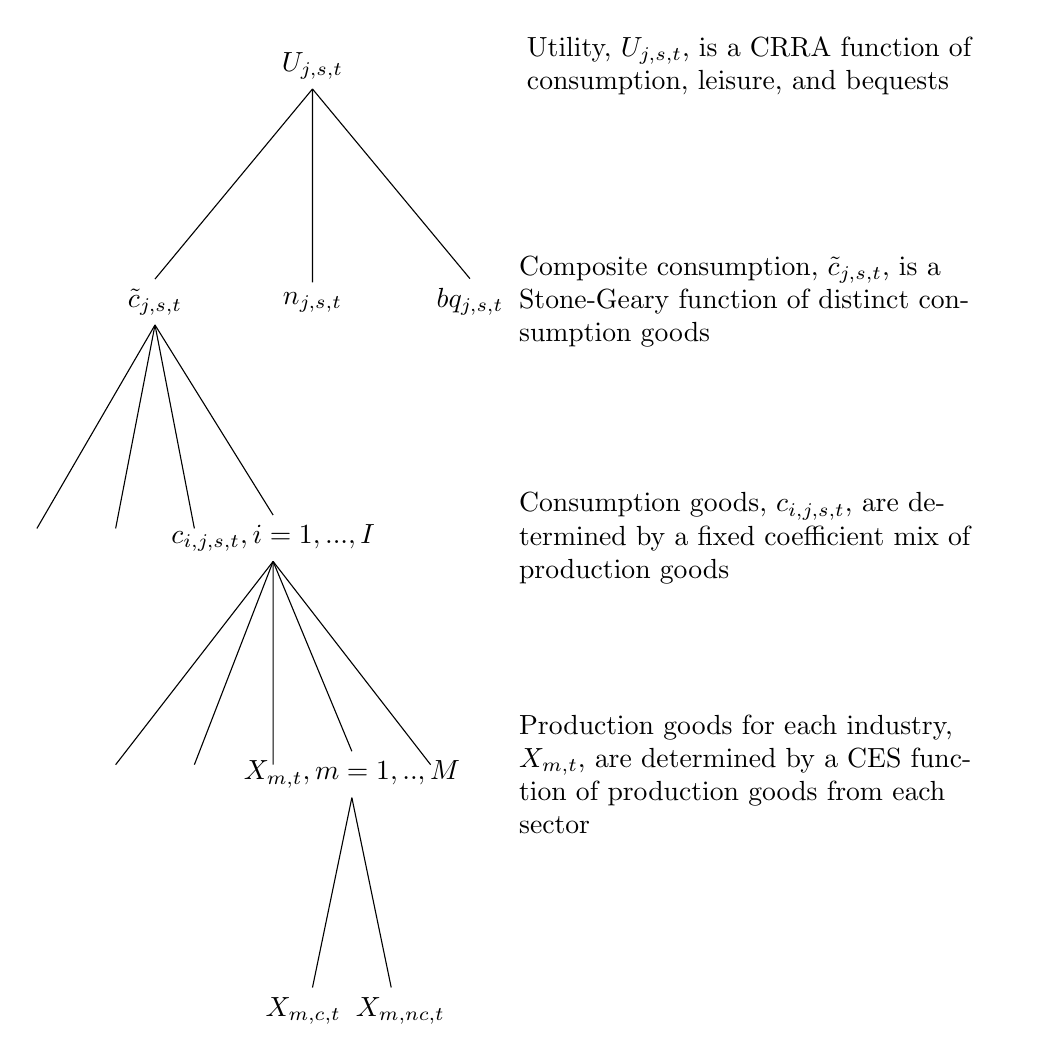
\begin{tikzpicture}
\tikzstyle{every node}=[auto,every node/.style={rectangle,draw, text centered, text width=1.3cm,minimum height=0.8cm },node distance=3cm]
\tikzset{%
level 1/.style={sibling distance = 2cm, level distance=3cm,edge from parent path={(\tikzparentnode.south) -- (\tikzchildnode.north)}},
level 2/.style={sibling distance = 1cm,level distance=3cm}
%level 4/.style={sibling distance = 1.1cm,level distance=3cm}
}
  \node (0){$U_{j,s,t}$}
    child {node (1) {$\tilde{c}_{j,s,t}$}
    child {node {}}
    child {node {}}
    child {node {}}
    child {node (2){$c_{i,j,s,t}, i=1,...,I$}   
child {node (3) {}}
            child {node {}}
            child {node {}}
            child {node {$X_{m,t}, m=1,..,M$}       
             child {node {$X_{m,c,t} \ \ $}}
             child {node {$\ \ X_{m,nc,t}$}}}
             child {node {}}
                        }
                  }
child {node {$n_{j,s,t}$}}
child {node {$bq_{j,s,t}$}} ;

\node at (0) [xshift=+2.6cm,right,draw=none, text width=6cm]{Utility, $U_{j,s,t}$, is a CRRA function of consumption, leisure, and bequests};
\node at (1) [xshift=+4.5cm, right,draw=none, text width=6cm]{Composite consumption, $\tilde{c}_{j,s,t}$, is a Stone-Geary function of distinct consumption goods};
\node at (2) [xshift=+3.0cm, right,draw=none, text width=6cm]{Consumption goods, $c_{i,j,s,t}$, are determined by a fixed coefficient mix of production goods };
\node at (3) [xshift=+5.0cm, right,draw=none, text width=6cm]{Production goods for each industry, $X_{m,t}$, are determined by a CES function of production goods from each sector};
\end{tikzpicture}
\end{figure}


    Households choose consumption of a composite consumption good, $c_{j,s+u,t+u}$, labor supply, $n_{j,s+u,t+u},$ and asset holdings, $b_{j,s+u+1,t+u+1}$, to maximize the expected, discounted, lifetime utility subject to their per-period budget constraint.  Total consumption of the composite good is made up of discretionary consumption, $\tilde{c}_{j,s,t}$, and minimum required purchases of each consumption good, $\bar{c}_{i,s}$.  Thus the consumer's choice is over $\tilde{c}_{j,s,t}$, which together with the minimum required purchases equal determine total composite consumption: $c_{j,s,t}=\tilde{c}_{j,s,t}+\sum_{i=1}^{I}c_{i,s}$.  It is therefore the case that there minimum required purchases affect the household's ability to smooth consumption over time.  We discuss the composite consumption good in more detail in Section \ref{sec:subutil}.  This composite good is age dependent, thus the price of the composite consumption good varies with age $s$.  We denote the gross-of-tax price of the composite consumption good for households of age $s$ in period $t$ as $\tilde{p}_{s,t}$ and the gross-of-tax price for good $i$ at time $t$ as $p_{i,t}$. The households' per period budget constraint is:
    
    \begin{equation}\label{EqBC}
      \begin{split}
        \sum_{i=1}^{I} p_{i,t}\bar{c}_{i,s} + \tilde{p}_{s,t}\tilde{c}_{s,t} + b_{j,s+1,t+1} \leq \left(1 + r_t\right) b_{j,s,t} + w_t e_{j,s}&n_{j,s,t} + \frac{BQ_{j,t}}{\lambda_j\tilde{N}_t} - T_{j,s,t} \\
        \quad\text{where}\quad b_{j,s,1} = 0 \\
        &\text{for} \quad E+1\leq s \leq E+S \quad \forall j,t
      \end{split}
    \end{equation}

\noindent\noindent Here, $r_{t}$ and $w_{t}$ are the real interest rate and the wages rate on a unit of effective labor.  The variable $e_{j,s}$ denotes the effective labor units of an individual from lifetime income group $s$ and age $j$.  An individual's labor income is thus determined by her choice of $n_{j,s,t}$ units of labor times her measure of effective labor units, $e_{j,s}$, times the wage per unit of effect labor.  An individuals effective labor units vary over the life-cycle, as the age subscript implies.  $BQ_{j,t}$ denote aggregate bequests left from those in lifetime income group {j} at time {t}.  We divide this number by the number of individuals in lifetime income group $j$ at time $t$, given by $\lambda_{j}\tilde{N}_{t}$, to determine the amount of bequests received by each household in lifetime income group $j$.\footnote{This distribution of bequests is just place holder. The goal is to find suitable data to calibrate the process describing the transmission of bequests between individuals of different ages and lifetime income groups.}  The last term in the budget constraint, $T_{j,s,t}$ are total taxes paid by the individual.  These include all non-consumption taxes and are based on tax functions for separate tax sources that we estimate based on a microsimulation model.  We discuss the parameterization and calibration of these functions below. 

    The Lagrangian for the individual's problem can be written as:
     \begin{equation}\label{eqn:hh_prob_lagrangian}
      \begin{split}
     \mathcal{L} =  \max_{\left\{ \substack{\tilde{c}_{j,s+u,t+u},\\\ {n}_{j,s+u,t+u},\\\ {b}_{j,s+u,t+u}}\right\}_{u=0}^{E+S-s}}  &  \sum_{u=0}^{E+S-s}\beta^u\left[\prod_{v=s-1}^{s+u-1}(1-\rho_v)\right]  \frac{\left(c_{j,s+u,t+u}\right)^{1-\sigma} - 1}{1-\sigma} + ...\\
  &   e^{g_y t(1-\sigma)}\chi^n_s+u\left(b\left[1 - \left(\frac{n_{j,s+u,t+u}}{\tilde{l}}\right)^\upsilon\right]^\frac{1}{\upsilon} + k\right) + \rho_s\chi^b\frac{\left(b_{j,s+u+1,t+u+1}\right)^{1-\sigma} - 1}{1-\sigma}  +... \\
       & \lambda_{j,s+u,t+u}\left\{ (1+r_{t+u})b_{j,s+u,t+u} + w_{t+u}e_{j,s+u}n_{j,s+u,t+u}+\frac{BQ_{j,t+u}}{\lambda_{j}\tilde{N}_{t+u}}-T_{j,s+u,t+u} -.... \right.\\
       & \left. \sum_{i=1}^{I}p_{i,t+u}\bar{c}_{i,s+u}-\tilde{p}_{s+u,t+u}\tilde{c}_{j,s+u,t+u} -b_{j,s+u+1,t+u+1} \right\}
        \end{split}
    \end{equation}
    
    
    
\noindent\noindent taking derivatives with respect to $\{\tilde{c}_{j,s,t},n_{j,s,t+u},b_{j,s,t+1}\}$ gives us the necessary conditions for each $j,s$ and $t$.  The necessary condition with respect to the discretionary consumption of the composite consumption good, $\tilde{c}_{j,s+u,t+u}$, labor supply, $n_{j,s+u,t+u}$, and asset holdings, $b_{j,s+u+1,t+u+1}$, are:
  
    \begin{equation}\label{Eqcfoc}
      \begin{split}
     \frac{\partial U}{\partial \tilde{c}_{j,s+u,t+u}}  = \beta^u\left[\prod_{v=s-1}^{s+u-1}(1-\rho_v)\right] c_{j,s+u,t+u}^{-\sigma} - \beta^u\left[\prod_{v=s-1}^{s+u-1}(1-\rho_v)\right]  \lambda_{j,s+u,t+u} \tilde{p}_{s+u,t+u} = 0, \forall u
        \end{split}
    \end{equation}

    \begin{equation}\label{Eqnfoc}
      \begin{split}
      \frac{\partial U}{\partial n_{j,s+u,t+u}} & = \beta^u\left[\prod_{v=s-1}^{s+u-1}(1-\rho_v)\right] e^{g_y (t+u)(1-\sigma)}\chi^n_{s}\biggl(\frac{b}{\tilde{l}}\biggr)\biggl(\frac{n_{j,s+u,t+u}}{\tilde{l}}\biggr)^{v-1}\Biggl[1 - \biggl(\frac{n_{j,s+u,t+u}}{\tilde{l}}\biggr)\Biggr]^{\frac{1-v}{v}} \\
      & -  \beta^u\left[\prod_{v=s-1}^{s+u-1}(1-\rho_v)\right]\lambda_{j,s+u,t+u} \left( w_{t+u} e_{j,s+u} - \frac{\partial T_{j,s+u,t+u}}{\partial n_{j,s+u,t+u}} \right)= 0, \forall u
        \end{split}
    \end{equation}

    \begin{equation}\label{Eqbfoc}
      \begin{split}
      \frac{\partial U}{\partial b_{j,s+u+1,t+u+1}} & = \beta^u\left[\prod_{v=s-1}^{s+u-1}(1-\rho_v)\right] \rho_s\chi^b\bigl(b_{j,s+u+1,t+u+1}\bigr)^{-\sigma} - \beta^u\left[\prod_{v=s-1}^{s+u-1}(1-\rho_v)\right] \lambda_{j,s+ut+u}  \\\ 
      & + \beta^{u+1}\left[\prod_{v=s-1}^{s+u}(1-\rho_v)\right] \lambda_{j,s+u+1,t+u+1} \left( 1 + r_{t+u+1} - \frac{\partial T_{j,s+u+1,t+u+1}}{\partial b_{j,s+u+1,t+u+1}} \right)= 0, \forall u
      \end{split}
    \end{equation}

 Note that the term $\frac{\partial T_{j,s+u+1,t+u+1}}{\partial n_{j,s+U+1,t+u+1}}$ give the change in total taxes for additional labor supply $\frac{\partial T_{j,s+u+1,t+u+1}}{\partial b_{j,s+U+1,t+u+1}}$ gives the change in total taxes for additional savings.  The tax functions that define the total taxes paid will take into account the interactions, for example how increasing capital income by saving more impacts the marginal tax rate on labor income in a system that progressively taxes labor income.  Rearranging the equations above to solve each for $\lambda_{t+u}$, we get the following:
    \begin{equation}
      \begin{split}
      \lambda_{j,s+u,t+u} = \frac{c_{j,s+u,t+u}^{-\sigma}}{\tilde{p}_{s,t+u}} \nonumber
      \end{split}
    \end{equation}

    \begin{equation}
      \begin{split}
      \lambda_{j,s+u,t+u} = \frac{e^{g_y (t+u)(1-\sigma)}\chi^n_{s}\biggl(\frac{b}{\tilde{l}}\biggr)\biggl(\frac{n_{j,s+u,t+u}}{\tilde{l}}\biggr)^{v-1}\Biggl[1 - \biggl(\frac{n_{j,s+u,t+u}}{\tilde{l}}\biggr)\Biggr]^{\frac{1-v}{v}}}{ w_{+u} e_{j,s+u} - \frac{\partial T_{j,s+u,t+u}}{\partial n_{j,s+u,t+u}} }  \nonumber
      \end{split}
    \end{equation}

    \begin{equation}
      \begin{split}
      \lambda_{j,s+u,t+u} = \rho_s\chi^b\bigl(b_{j,s+u+1,t+u+1}\bigr)^{-\sigma} - \beta (1-\rho_{s+u}) \lambda_{t+u+1} \left( 1 + r_{t+u+1} - \frac{\partial T_{j,s+u+1,t+u+1}}{\partial b_{j,s+u+1,t+u+1}} \right)
        \end{split}  \nonumber
    \end{equation}

    These three equations can then be reduced to just two equations that must hold for all $j,s,$ and $t$.  The first relates the marginal utility of consumption of the composite good to the marginal utility of labor:
    \begin{equation}\label{EqcEuler}
      \begin{split}
      & \frac{ c_{j,s+u,t+u}^{-\sigma}}{\tilde{p}_{s+u,t+u}} \\
      & = \frac{ e^{g_y (t+u)(1-\sigma)}\chi^n_{s}\biggl(\frac{b}{\tilde{l}}\biggr)\biggl(\frac{n_{j,s+u,t+u}}{\tilde{l}}\biggr)^{v-1}\Biggl[1 - \biggl(\frac{n_{j,s+u,t+u}}{\tilde{l}}\biggr)\Biggr]^{\frac{1-v}{v}} } { w_{t+u} e_{j,s+u} - \frac{\partial T_{j,s+u,t+u}}{\partial n_{j,s+u,t+u}} }
       \end{split}
    \end{equation}

    \noindent\noindent The second equation is the intertemporal Euler equation for savings, including the utility effects of bequests:
    \begin{equation}\label{EqbEuler}
      \begin{split}
      & \frac{ c_{j,s+u,t+u}^{-\sigma}}{\tilde{p}_{s+u,t+u}} = \rho_s\chi^b\bigl(b_{j,s+U+1,t+U+1}\bigr)^{-\sigma}  + \frac{ \beta(1-\rho_{s+u}) c_{j,s+u+1,t+u+1}^{-\sigma}} {\tilde{p}_{s+u+1,t+u+1}} \times \left( 1 + r_{t+u+1} - \frac{\partial T_{j,s+u+1,t+U+1}}{\partial b_{j,s+u+1,t+u+1}} \right)
      \end{split}
    \end{equation}

       
    \subsection{Household's Subutility Function}\label{sec:subutil}
    
    Household preferences over the composite consumption good are modeled as a Stone-Geary function. The aggregate discretionary consumption of the composite good is defined as follows.
    \begin{equation} \label{eqn:comp_cons}
        \tilde{c}_{j,s,t}  = \prod_{i=1}^I \left( c_{i,j,s,t} - \bar c_{i,s} \right) ^{\alpha_{i,s}} 
    \end{equation}

Where, $c_{i,j,s,t}$ is consumption of good $i$ by household of type $j$, age $s$, at time $t$.  There are $I$ total goods and $\bar{c}_{i,s}$ represents the minimum consumption amount for each good at each age.  The parameters $\alpha_{i,s}$ are the share parameters (and $\sum_{i=1}^{I} \alpha_{i,s}=1$).  They correspond to the share of income, after minimum expenditure amounts, that are spent on each good at each age.  Allowing the minimum consumption amounts and the share parameters to vary by age helps to incorporate life-cycle profiles of consumption into the model.  For example, we do not explicitly model household formation decisions, but they will be some of the effects of changes in household composition over the life-cycle are obtained through the parameters of the Stone-Geary function.  For example, the minimum required expenditure on shelter may be higher in the middle of the life-cycle when household size is larger.  The minimum consumption amounts also mean that the composition of consumption will vary with income, even though all households have the same utility function.

The consumer chooses $c_{i,j,s,t}$ to maximize Equation \ref{Eqcagg} subject to the budget constraint:

    \begin{equation} \label{eqn:cons_budgetcons}
        \sum_{i=1}^{I} p_{i,t}(c_{i,j,s,t}-\bar{c}_{i,s})  = \tilde{p}_{s,t}\tilde{c}_{j,s,t}
    \end{equation}

\noindent where $p_{i,t}$ is the gross of tax price of good $i$ at time $t$ and $\tilde{p}_{s,t}$ is the gross of tax price of the the discretionary component of the composite consumption good consumed by those of age $s$ at time $t$.  Maximization of \ref{Eqcagg} subject to \ref{eqn:cons_budgetcons} yields:

    \begin{equation} \label{eqn:cons_lagrangian}
       \mathcal{L} =  \max_{\{c_{i,j,s,t}\}_{i=1}^{I}}  \prod_{i=1}^I \left( c_{i,j,s,t} - \bar c_{i,s} \right) ^{\alpha_{i,s}}  + \lambda \left(\tilde{p}_{s,t}\tilde{c}_{j,s,t} - \sum_{i=1}^{I} p_{i,t}(c_{i,j,s,t}-\bar{c}_{i,j,s,t})\right)
    \end{equation}
    
    Which as $I$ FOCs (for each $j$, $s$, $t$):
    
      \begin{equation} \label{eqn:cons_FOC}
      \begin{split}
       & \frac{\partial \mathcal{L}}{\partial c_{i,j,s,t}} = \frac{\alpha_{i,s} \prod_{i=1}^I \left( c_{i,j,s,t} - \bar c_{i,s} \right) ^{\alpha_{i,s}}}{(c_{i,j,s,t}-\bar{c}_{i,s})}-\lambda p_{i,t} = 0, \forall \ i  \\
       & \implies  \frac{\alpha_{i,s} \prod_{i=1}^I \left( c_{i,j,s,t} - \bar c_{i,s} \right) ^{\alpha_{i,s}}}{(c_{i,j,s,t}-\bar{c}_{i,s})} = \lambda p_{i,t}, \forall \ i \\
       & \implies  \frac{\alpha_{i,s} \prod_{i=1}^I \left( c_{i,j,s,t} - \bar c_{i,s} \right) ^{\alpha_{i,s}}}{ p_{i,t}(c_{i,j,s,t}-\bar{c}_{i,s})} = \lambda, \forall \ i \\
       & \implies \frac{\alpha_{i,s}}{p_{i,t}(c_{i,j,s,t}-\bar{c}_{i,s})}=\frac{\alpha_{j,s}}{p_{k,t}(c_{k,j,s,t}-\bar{c}_{k,s})}, \forall \ i,k \\
       & \implies c_{i,j,s,t}= \frac{\alpha_{i,s} p_{k,t}(c_{k,j,s,t}-\bar{c}_{k,s})}{\alpha_{k,s} p_{i,t}} + \bar{c}_{i,s} \forall i,k 
       \end{split}
    \end{equation}
    
    Now substitute the last line of \ref{eqn:cons_FOC} into the budget constraint (Equation \ref{eqn:cons_budgetcons}):
    
          \begin{equation} \label{eqn:cons_solve}
      \begin{split}
       & \tilde{p}_{s,t}\tilde{c}_{j,s,t} = \sum_{i=1}^{I}p_{i,t}(c_{i,j,s,t}-\bar{c}_{i,s}) \\
       & \implies  \tilde{p}_{s,t}\tilde{c}_{j,s,t} = \sum_{i=1}^{I}p_{i,t}\left[ \frac{\alpha_{i,s} p_{k,t}(c_{k,j,s,t}-\bar{c}_{k,s})}{\alpha_{k,s} p_{i,t}} + \bar{c}_{i,s}- \bar{c}_{i,s}\right] \\
       & \implies  \tilde{p}_{s,t}\tilde{c}_{j,s,t} = \sum_{i=1}^{I}\left[ \frac{\alpha_{i,s} p_{k,t}(c_{k,s}-\bar{c}_{k,s})}{\alpha_{k,s}}\right] \\
       & \implies  \tilde{p}_{s,t}\tilde{c}_{j,s,t} = \frac{ p_{k,t}(c_{k,j,s,t}-\bar{c}_{k,s})}{\alpha_{k,s}} \underbrace{\sum_{i=1}^{I}\alpha_{i,s}}_{=1} \\	
        & \implies  \tilde{p}_{s,t}\tilde{c}_{j,s,t} = \frac{ p_{k,t}(c_{k,j,s,t}-\bar{c}_{k,s})}{\alpha_{k,s}} \\
        & \implies  \frac{ p_{k,t}(c_{k,j,s,t}-\bar{c}_{k,s})}{\alpha_{k,s}}  = \tilde{p}_{s,t}\tilde{c}_{j,s,t}   \\	
        & \implies  c_{k,j,s,t}  = \frac{\alpha_{k,s} \tilde{p}_{s,t}\tilde{c}_{j,s,t}}{p_{k,t}} + \bar{c}_{k,s},  \forall \ k  \\	
       \end{split}
    \end{equation}
    
    Thus, total consumption of each good $i$, $c_{i,j,s,t}$, is given by the the amount of minimum consumption plus the share of total expenditures remaining after making the minimum expenditures on all goods (this is called the ``supernumerary" expenditure).  We derive the prices of the age $s$ composite consumption good in period $t$, $\tilde{p}_{s,t}$ by using the demand for good $i$ provided in Equation \ref{cons_solve} in the function defining aggregate discretionary consumption, Equation \ref{eqn:comp_cons}: 
    
              \begin{equation} \label{eqn:composite_price}
      \begin{split}
      & \tilde{c}_{j,s,t} = \prod_{i=1}^{I}(c_{i,j,s,t}-\bar{c}_{i,s})^{\alpha_{i,s}} \\
      &\implies \tilde{c}_{j,s,t} = \prod_{i=1}^{I}\left( \frac{\alpha_{i,s} \tilde{p}_{s,t}\tilde{c}_{j,s,t}}{p_{i,t}} + \bar{c}_{i,s}-\bar{c}_{i,s}\right)^{\alpha_{i,s}} \\
      &\implies \tilde{c}_{j,s,t} = \prod_{i=1}^{I} \left( \frac{\alpha_{i,s} \tilde{p}_{s,t}\tilde{c}_{j,s,t}}{p_{i,t}} \right)^{\alpha_{i,s}} \\
      &\implies \tilde{c}_{j,s,t} =  \tilde{p}_{s,t}\tilde{c}_{j,s,t} \prod_{i=1}^{I}\left( \frac{\alpha_{i,s}}{p_{i,t}} \right)^{\alpha_{i,s}} \\
      &\implies \frac{\tilde{p}_{s,t}\tilde{c}_{j,s,t}}{\tilde{c}_{j,s,t}} =  \prod_{i=1}^{I}\left( \frac{p_{i,t}}{\alpha_{i,s}} \right)^{\alpha_{i,s}} \\
       &\implies \tilde{p}_{s,t} =  \prod_{i=1}^{I}\left( \frac{p_{i,t}}{\alpha_{i,s}} \right)^{\alpha_{i,s}} \\
       \end{split}
    \end{equation}
    
    This composite good price is then used in the household's intertemporal optimization problem described in Equation \ref{eqn:hh_prob_lagrangian}.  With the parameters and endogenous variables, we then use \ref{eqn:cons_solve} to find the $c_{i,j,s,t}$.
    
    \subsection{Relating Consumption and Production Goods}\label{sec:prod_cons_map}
    
    Our model contains $I$ consumption goods and $M$ production goods.  We denote the quantity of production good $m$ in period $t$ as $X_{m,t}$.  We relate the output of the production sectors and the consumption goods using a fixed coefficient model. That is, we assume each consumption good is made up of a mix of the outputs of different production sectors.  This means that the composition of these consumption goods do not respond to prices. The weights that determine the mix for each consumption goods are given in the matrix $\Pi$.  Element $\pi_{i,m}$ of the matrix $\Pi$ corresponds to the percentage contribute of the output of sector $m$ in the production of good $i$.  The total supply of good $i$ in the economy at time $t$ is thus given by: 
    
             \begin{equation} \label{eqn:mix_cons}
             c_{i,t} = \sum_{m=1}^{M}\pi_{i,m}X_{m,t} 
    	\end{equation}
	
 \noindent\noindent And the price of a unit of consumption good $i$ at time $t$ is:
	
             \begin{equation} \label{eqn:mix_cons_price}
             p_{i,t} = \sum_{m=1}^{M}\pi_{i,m}p_{m,t}, 
    	\end{equation}
    
    \noindent\noindent Where $p_{m}$ is the price of output of production sector $m$ at time $t$.
    
    \subsection{Preferences for Corporate vs. Noncorporate Goods}\label{sec:pref_corp_noncorp}
    
    Production sectors may contain corporate and non-corporate producers, each facing different tax treatment.  If the output from corporate and non-corporate entities are perfect substitutes, then if the producers have the same production technology, consumers will end up consuming only the output from the sector with lowest after tax cost of producing.  \citet{GK1989} propose a model where different production sectors use different technologies, which can give rise to an equilibrium where both the corporate and non-corporate sector produce the same good.  We take a different track, following \citet{FR1993} we allow production technologies to vary across industry, but not across sectors within industry.  Both sectors produce output in equilibrium, because output across sectors are not perfect substitutes.  For example, food outside the home from a corporate, chain restaurant chain is not the same as food outside the home from a small, family-owned restaurant.  Specifically, we define consumer preferences such that demand for the composite production good (combing output from the corporate and non-corporate sector) for production sector $m$ at time $t$, $X_{m,t}$, is a constant elasticity of substitution (CES) function of the output from the corporate and non-corporate sectors, $X_{m,t,C}$ and $X_{m,t,NC}$, respectively:
    
                  \begin{equation} \label{eqn:comp_output}
             X_{m,t} = \left[\gamma_{m}^{\frac{1}{\ve_{3}}}X_{m,t,C}^{\frac{(\ve_{3}-1)}{\ve_{3}}}+(1-\gamma_{m})^{\frac{1}{\ve_{3}}}X_{m,t,NC}^{\frac{(\ve_{3}-1)}{\ve_{3}}}+\right]^{\frac{\ve_{3}}{(\ve_{3}-1)}}, 
    	\end{equation}
	
	\noindent where $\ve_{3}$ is the elasticity of substitution between corporate and non-corporate output and is assumed to be constant across industries.  The share parameter in the CES function, $\gamma_{m}$ is allowed to vary across industry and will be identified by the fraction of corporate produced output across industries.  The CES function thus explains the existence of corporate and non-corporate production within each industry as well as the different shares of corporate output across industries.  Because of these preferences, changes in corporate and non-corproate tax treatment will have differential impacts across consumers of different ages and income levels.  
	Consumers choose $X_{m,t,C}$ and $X_{m,t,NC}$ to maximize \ref{eqn:comp_output} subject to:
	
	 \begin{equation} \label{eqn:comp_output_cons}
             p_{m,t}X_{m,t} = p_{m,t,C}X_{m,t,C}+p_{m,t,NC}X_{m,t,NC}, 
    	\end{equation}
	
	
\noindent where $p_{m,t,C}$ and $p_{m,t,NC}$ are the prices of output from the corporate and non-corporate firms in production industry $m$, respectively.  Note that these prices are determined through the firm's profit maximization problem and the zero economic profit condition for firms. The constrained optimization problem consumers face is: 
    
 \begin{equation} \label{eqn:comp_output_lagrangian}
	\begin{split}
	 \mathcal{L} = \left[\gamma_{m}^{\frac{1}{\ve_{3}}}X_{m,t,C}^{\frac{(\ve_{3}-1)}{\ve_{3}}}+(1-\gamma_{m})^{\frac{1}{\ve_{3}}}X_{m,t,NC}^{\frac{(\ve_{3}-1)}{\ve_{3}}}+\right]^{\frac{\ve_{3}}{(\ve_{3}-1)}} + \lambda_{m,t,C}\left(p_{m,t}X_{m,t} - p_{m,t,C}X_{m,t,C}+p_{m,t,NC}X_{m,t,NC}\right)
  	\end{split}
\end{equation}
    
    FOCs are:
    
\begin{equation} \label{eqn:comp_output_foc_C}
	\begin{split}
       	&  \frac{\partial \mathcal{L}}{\partial X_{m,t,C}} = \gamma_{m}^{\frac{1}{\ve_{3}}} X_{m,t,C}^{\frac{-1}{\ve_{3}}} \left[\gamma_{m}^{\frac{1}{\ve_{3}}}X_{m,t,C}^{\frac{(\ve_{3}-1)}{\ve_{3}}}+(1-\gamma_{m})^{\frac{1}{\ve_{3}}}X_{m,t,NC}^{\frac{(\ve_{3}-1)}{\ve_{3}}}+\right]^{\frac{1}{(\ve_{3}-1)}} - \lambda_{m,t,C} p_{m,t,C} = 0
      	 \end{split}
\end{equation}
    
   and
   
\begin{equation} \label{eqn:comp_output_foc_NC}
	\begin{split}
       	&  \frac{\partial \mathcal{L}}{\partial X_{m,t,NC}} = (1-\gamma_{m})^{\frac{1}{\ve_{3}}} X_{m,t,NC}^{\frac{-1}{\ve_{3}}} \left[\gamma_{m}^{\frac{1}{\ve_{3}}}X_{m,t,C}^{\frac{(\ve_{3}-1)}{\ve_{3}}}+(1-\gamma_{m})^{\frac{1}{\ve_{3}}}X_{m,t,NC}^{\frac{(\ve_{3}-1)}{\ve_{3}}}+\right]^{\frac{1}{(\ve_{3}-1)}} - \lambda_{m,t,C} p_{m,t,NC} = 0
	\end{split}
\end{equation}
    
    Solving the two necessary conditions, we can find the equations for the demand for the corporate and non-corporate output in industry $m$ as a function of the prices out output from each sector of industry $m$, price of the composite production good, the demand for the composite production good, and the parameters:
    
\begin{equation} \label{eqn:demand_XmtC}
	X_{m,t,C} = \frac{\gamma_{m}p_{m,t}X_{m,t}}{p_{m,t,C}^{\ve_{3}}\left[\gamma_{m}p_{m,t,C}^{1-\ve_{3}}+(1-\gamma_{m})p_{m,t,NC}^{1-\ve_{3}}\right]}
\end{equation}
    
    and 
    
    \begin{equation} \label{eqn:demand_XmtNC}
	X_{m,t,NC} = \frac{(1-\gamma_{m})p_{m,t}X_{m,t}}{p_{m,t,NC}^{\ve_{3}}\left[\gamma_{m}p_{m,t,C}^{1-\ve_{3}}+(1-\gamma_{m})p_{m,t,NC}^{1-\ve_{3}}\right]}
\end{equation}

To determine $p_{m,t}$, note that the CES subutility function defining preferences over corporate and non-corporate output within a production industry is linearly homogenous.  Because the subutility function is linearly homogenous, we know that the associated indirect utility function is homogenous of degree one in $X_{m,t}$.  Letting $V(\cdot)$ represent the indirect utility function, this means that $V(p_{m,t,C},p_{m,t,NC},\lambda X_{m,t}) = \lambda V(p_{m,t,C},p_{m,t,NC}, X_{m,t})$.  The linear homogeneity of the utility function also means that the indirect utility function is homogenous of degree -1 in prices.  That is, $V(\lambda p_{m,t,C},\lambda p_{m,t,NC}, X_{m,t}) = \frac{V(p_{m,t,C},p_{m,t,NC}, X_{m,t})}{\lambda}$. Linear homogeneity of the utility function means that: 

\begin{equation}
V(p_{m,t,C},p_{m,t,NC}, X_{m,t}) = \frac{p_{m,t}X_{m,t}}{e(p_{m,t,C},p_{m,t,NC})},
\end{equation}
    
    
\noindent\noindent where $e(p_{m,t,C},p_{m,t,NC})$ is the minimum expenditure for a unit of the composite good given prices.  Rearranging, we have: 
    
 \begin{equation}
 \label{eqn:price_comp}
 \begin{split}
& e(p_{m,t,C},p_{m,t,NC}) = \frac{p_{m,t}X_{m,t}}{V(p_{m,t,C},p_{m,t,NC}, X_{m,t})}\\
&\implies e(p_{m,t,C},p_{m,t,NC}) = p_{m,t}X_{m,t}/ \\
& {\left[\gamma_{m}^{\frac{1}{\ve_{3}}}\left( \frac{\gamma_{m}p_{m,t}X_{m,t}}{p_{m,t,C}^{\ve_{3}}\left[\gamma_{m}p_{m,t,C}^{1-\ve_{3}}+(1-\gamma_{m})p_{m,t,NC}^{1-\ve_{3}}\right]}\right)^{\frac{(\ve_{3}-1)}{\ve_{3}}}+(1-\gamma_{m})^{\frac{1}{\ve_{3}}}\left(\frac{(1-\gamma_{m})p_{m,t}X_{m,t}}{p_{m,t,NC}^{\ve_{3}}\left[\gamma_{m}p_{m,t,C}^{1-\ve_{3}}+(1-\gamma_{m})p_{m,t,NC}^{1-\ve_{3}}\right]}\right)^{\frac{(\ve_{3}-1)}{\ve_{3}}}+\right]^{\frac{\ve_{3}}{(\ve_{3}-1)}}}\\
&\implies e(p_{m,t,C},p_{m,t,NC}) = p_{m,t}X_{m,t}/ \\
& {p_{m,t}X_{m,t}\left[\gamma_{m}^{\frac{1}{\ve_{3}}}\left( \frac{\gamma_{m}}{p_{m,t,C}^{\ve_{3}}\left[\gamma_{m}p_{m,t,C}^{1-\ve_{3}}+(1-\gamma_{m})p_{m,t,NC}^{1-\ve_{3}}\right]}\right)^{\frac{(\ve_{3}-1)}{\ve_{3}}}+(1-\gamma_{m})^{\frac{1}{\ve_{3}}}\left(\frac{(1-\gamma_{m})}{p_{m,t,NC}^{\ve_{3}}\left[\gamma_{m}p_{m,t,C}^{1-\ve_{3}}+(1-\gamma_{m})p_{m,t,NC}^{1-\ve_{3}}\right]}\right)^{\frac{(\ve_{3}-1)}{\ve_{3}}}+\right]^{\frac{\ve_{3}}{(\ve_{3}-1)}}}\\
&\implies e(p_{m,t,C},p_{m,t,NC}) = 1/ \\
& \left[\gamma_{m}p_{m,t,C}^{1-\ve_{3}}+(1-\gamma_{m})p_{m,t,NC}^{1-\ve_{3}}\right]{\left[\gamma_{m}^{\frac{1}{\ve_{3}}}\left( \frac{\gamma_{m}}{p_{m,t,C}^{\ve_{3}}}\right)^{\frac{(\ve_{3}-1)}{\ve_{3}}}+(1-\gamma_{m})^{\frac{1}{\ve_{3}}}\left(\frac{(1-\gamma_{m})}{p_{m,t,NC}^{\ve_{3}}}\right)^{\frac{(\ve_{3}-1)}{\ve_{3}}}+\right]^{\frac{\ve_{3}}{(\ve_{3}-1)}}}\\
&\implies e(p_{m,t,C},p_{m,t,NC}) = 
\frac{\left[\gamma_{m}^{\frac{1}{\ve_{3}}}\left( \frac{\gamma_{m}}{p_{m,t,C}^{\ve_{3}}}\right)^{\frac{(\ve_{3}-1)}{\ve_{3}}}+(1-\gamma_{m})^{\frac{1}{\ve_{3}}}\left(\frac{(1-\gamma_{m})}{p_{m,t,NC}^{\ve_{3}}}\right)^{\frac{(\ve_{3}-1)}{\ve_{3}}}+\right]^{\frac{\ve_{3}}{(1-\ve_{3})}}}{\left[\gamma_{m}p_{m,t,C}^{1-\ve_{3}}+(1-\gamma_{m})p_{m,t,NC}^{1-\ve_{3}}\right]}\\
&\implies e(p_{m,t,C},p_{m,t,NC}) = 
\frac{\left[\gamma_{m}\left( \frac{1}{p_{m,t,C}^{\ve_{3}}}\right)^{\frac{(\ve_{3}-1)}{\ve_{3}}}+(1-\gamma_{m})\left(\frac{1}{p_{m,t,NC}^{\ve_{3}}}\right)^{\frac{(\ve_{3}-1)}{\ve_{3}}}+\right]^{\frac{\ve_{3}}{(1-\ve_{3})}}}{\left[\gamma_{m}p_{m,t,C}^{1-\ve_{3}}+(1-\gamma_{m})p_{m,t,NC}^{1-\ve_{3}}\right]}\\
&\implies e(p_{m,t,C},p_{m,t,NC}) = 
\frac{\left[\gamma_{m}p_{m,t,C}^{1-\ve_{3}}+(1-\gamma_{m})p_{m,t,NC}^{1-\ve_{3}}\right]^{\frac{\ve_{3}}{(1-\ve_{3})}}}{\left[\gamma_{m}p_{m,t,C}^{1-\ve_{3}}+(1-\gamma_{m})p_{m,t,NC}^{1-\ve_{3}}\right]}\\
&\implies e(p_{m,t,C},p_{m,t,NC}) = 
\left[\gamma_{m}p_{m,t,C}^{1-\ve_{3}}+(1-\gamma_{m})p_{m,t,NC}^{1-\ve_{3}}\right]^{\frac{1}{(1-\ve_{3})}}\\
\end{split}
\end{equation}   

\noindent\noindent Thus we have the price of the corporate-non-corporate composite good from production industry $m$ at time $t$ as:
\begin{equation}
 e(p_{m,t,C},p_{m,t,NC})=p_{m,t}=\left[\gamma_{m}p_{m,t,C}^{1-\ve_{3}}+(1-\gamma_{m})p_{m,t,NC}^{1-\ve_{3}}\right]^{\frac{1}{(1-\ve_{3})}}
 \end{equation}
 
%\textcolor{red}{I'm not sure, but I think we then have  $e(p_{m,t,C},p_{m,t,NC})=p_{m,t}$ since the unit of ``utility" is really a unit of output of the composite production good, $X_{m,t}$}.


    
    

\chapter{Firms}
\index{Firms%
@\emph{Firms}}%



 \section{Supply Side Model Components: Variables and Parameters}
\label{sec:components}

\subsection{Variables}

There are six unique state variables, all of which are exogenous.  Note that $r_{s}$ is directly determined by $i_{s}$ and the tax rate on interest income.

% Table generated by Excel2LaTeX from sheet 'State Variables'
\begin{table}[htbp]
  \centering
  \caption{State Variables}
    \begin{tabular}{ll}
    \hline
    \hline
    Variable & Description \\
    \hline
    $K^{C}_{s}$ & Capital stock at the beginning of period $s$ \\
    $K^{\tau C}_{s-1}$ & Tax basis of the capital stock at the beginning of period $s$\\
    $B^{C}_{s}$ & Debt at the beginning of period $s$ \\
    $p^{C}_{s}$ & Price of corporate good in period $s$ \\
    $w_{s}$ & Wage rate in period $s$ \\
    $i_{s}$ & Nominal interest rate in period $s$ \\
    $r_{s}$ & After tax nominal rate of return in period $s$ \\
    \hline
    \hline
    \end{tabular}%
  \label{tab:state_vars}%
\end{table}%

Note in $K^{\tau C}_{s-1}$ the $s-1$ subscript - depreciation in period $s$ will be based on this and investment in period $s$.

There are 14 control variables, although all of these are trivial after the determination of $I^{C}_{s}$ and $EL^{C}_{s}$.

% Table generated by Excel2LaTeX from sheet 'Control Variables'
\begin{table}[htbp]
  \centering
  \caption{Control Variables}
    \begin{tabular}{lll}
    \hline
    \hline
    Variable & Description & Identifying Equation \\
    \hline
    $I^{C}_{s}$ & Firm investment in period $s$ & \ref{eqn:opt_i} \\
    $EL^{C}_{s}$ & Firm effective labor demand in period $s$ & \ref{eqn:foc_l} \\
    $X^{C}_{s}$ & Corp goods produced & \ref{eqn:prod_fun} \\
    $K^{C}_{s+1}$ & Firm's capital stock at the end of period $s$ (beginning of period $s+1$) & \ref{eqn:lom_capital} \\
    $EARN^{C}_{s}$ & Corp earnbefore deprec, corp taxes, and adjust costs, but after property taxes in period $s$ & \ref{eqn:earn} \\
    $DIV^{C}_{s}$ & Corporate dividends in period $s$ & \ref{eqn:div} \\
    $TE^{C}_{s}$ & Total corporate income taxes in period $s$ & \ref{eqn:corp_tax} \\
    $\Phi^{C}_{s}$ & Investment adjustment costs in period $s$ & \ref{eqn:adj_cost} \\
    $B^{C}_{s+1}$ & Corp debt at the end of period $s$ (start of period $s+1$) & \ref{eqn:debt} \\
    $K^{\tau C}_{s}$ & Tax basis of capital under corp income tax at end of period $s$ (beginning of $s+1$) & \ref{eqn:lom_taxcapital} \\
    $VN^{C}_{s}$ & New equity issued by the corp sector in period $s$ & \ref{eqn:vn} \\
    $V^{C}_{s}$ & Firm value in period $s$ & \ref{eqn:avg_q} \\
    $q^{C}_{s}$ & Marginal $q$ (change in firm value per dollar of investment) & \ref{eqn:foc_k} \\
    $Q^{C}_{s}$ & Average $Q$ & \ref{eqn:avg_q} \\
    \hline
    \hline
    \end{tabular}%
  \label{tab:control_vars}%
\end{table}%


\subsection{Parameters}

The model has 19 parameters.  Of these, 7 relate to the firm's production function, 2 to economic growth, 2 to firm financial policy, and 10 to tax policy.

% Table generated by Excel2LaTeX from sheet 'Parameters'
\begin{table}[htbp]
  \centering
  \caption{Model Parameters}
    \begin{tabular}{ll}
    \hline
    \hline
    Parameter & Description \\
    \hline
    Production Function &  \\
    \ \ \ $\gamma_{C}$ & Capital weighting in CES production function \\
    \ \ \ $\epsilon_{C}$ & Elasticity of substitution of capital for labor in CES production function \\
    \ \ \ $\delta^{C}$ & Rate of economic depreciation on capital stock in the corporate sector \\
    \ \ \ $\beta^{C}$ & Scaling parameter for quadratic investment adjustment costs \\
    \ \ \ $\mu_{C}$ & Steady-state investment rate \\
    Economic Growth &  \\
    \ \ \ $n$ & Rate of population growth (exogenous) \\
    \ \ \ $g$ & Rate of productivity growth (exogenous) \\
    Financial Policy &  \\
    \ \ \ $\zeta^{C}$ & Fraction of earnings paid out in dividends \\
    \ \ \ $b^{C}$ & Debt/Capital ratio \\
    Tax Policy &  \\
    \ \ \ $\tau^{b}_{s}$ & Corporate business income tax rate \\
    \ \ \ $\delta^{\tau C}_{s}$ & Rate of tax depreciation on corporate capital \\
    \ \ \ $\tau^{pC}_{s}$ & Property tax rate on corporate capital \\
    \ \ \ $\tau^{i}_{s}$ & Individual income tax rate on interest income \\
    \ \ \ $\tau^{g}_{s}$ & Individual income tax rate on capital gains \\
    \ \ \ $f_{e}$ & Dummy variable for full expensing of investment  \\
    \ \ \ $f_{i}$ & Dummy variable for deductibility of corporate interest paid \\
    \ \ \ $f_{p}$ & Dummy variable for deductibility of repayment of principle on loans \\
    \ \ \ $f_{b}$ & Dummy variable for inclusion of proceeds of loan in corp income tax base \\
    \ \ \ $f_{d}$ & Dummy variable for deductibility of depreciation expenses \\
    \hline
    \hline
    \end{tabular}%
  \label{tab:parameters}%
\end{table}%

\section{Necessary equations}
To solve the model, we want to get the optimal choices of labor and investment demand by firms.  Labor demand is determined through an intratemporal trade off between the costs and benefits of labor.  The necessary condition for the optimal choice of labor is: 

\begin{equation}
\label{eqn:foc_l}
p^{C}_{s}\frac{\partial F(K^{C}_{s},EL^{C}_{s})}{\partial EL^{C}_{s}}=w_{s}
\end{equation}

Investment is more complicated, as it presents an intertemporal tradeoff between the costs of investment today and the benefits of a higher capital stock tomorrow.  Once we have investment, all other endogenous variables follow from various accounting identities and assumptions on financial policies.

To derive the necessary conditions for investment, we need to first solve for the value of the firm as a function of the state variables (noted above) and the choice of investment. We do this by substituting in the various accounting identities to our equation for firm value.

Begin with the asset market equilibrium condition that the after-tax returns on all assets must be equalized if households simultaneously hold equity and bonds (and there is no aggregate uncertainty).  The after-tax, nominal return on holding bonds is:

\begin{equation}
\label{eqn:r}
r_{s}=(1-\tau^{i}_{s})i_{s},
\end{equation}

\noindent\noindent Where $i_{s}$ is the nominal interest rate on bonds.  Thus the return on holding corporate equity must equal $r_{s}$ in equilibrium:

\begin{equation}
\label{eqn:equity_eqm}
r_{s}=(1-\tau^{i}_{s})i_{s}=\frac{(1-\tau^{d}_{s})DIV^{C}_{s}+(1-\tau^{g}_{s})(V^{C}_{s+1}-V^{C}_{s}-VN^{C}_{s})}{V^{C}_{s}},
\end{equation}

where the first part of the numerator is the dividend returns from holding shares of the corporation and the second part are the capital gains returns from holding corporate equity, which are diluted by the issuance of new shares, $VN^{C}_{s}$.

We can rearrange this equation \ref{eqn:equity_eqm} to solve for $V^{C}_{s+1}$:

\begin{equation}
\label{eqn:v_s1}
\begin{split}
V^{C}_{s+1}&=\frac{V^{C}_{s}(1-\tau^{i}_{s})i_{s}-(1-\tau^{d}_{s})DIV^{C}_{s}}{(1-\tau^{g}_{s})}+V^{C}_{s}+VN^{C}_{s} \\
 & = V^{C}_{s}\underbrace{\left(1+\frac{(1-\tau^{i}_{s})i_{s}}{(1-\tau^{g}_{s})}\right)}_{\text{Let this be }1+\theta_{s}} + VN^{C}_{s} - \frac{(1-\tau^{d}_{s})}{(1-\tau^{g}_{s})}DIV^{C}_{s} \\
\end{split}
\end{equation}

\noindent\noindent Now we can solve this for $V^{c}_{s}$ by repeatedly substituting for $V^{C}_{s+1}$ and applying the transversality condition ($\lim_{T \to \infty} \prod_{t=1}^{T}(1+\theta_{t})V^{C}_{T}=0$):

\begin{equation}
\label{eqn:solve_vs}
\begin{split}
& V^{C}_{s}=\frac{V^{C}_{s+1}}{(1+\theta_{s})} - \frac{VN^{C}_{s}}{(1+\theta_{s})}  + \frac{\left(\frac{1-\tau^{d}_{s}}{1-\tau^{g}_{s}}\right)DIV^{C}_{s}}{(1+\theta_{s})} \\
\implies &  V^{C}_{s}=\frac{V^{C}_{s+2}}{(1+\theta_{s})(1+\theta_{s+1})} - \frac{VN^{C}_{s+1}}{(1+\theta_{s})(1+\theta_{s+1})}  + \frac{\left(\frac{1-\tau^{d}_{s}}{1-\tau^{g}_{s}}\right)DIV^{C}_{s+1}}{(1+\theta_{s})(1+\theta_{s+1})} - \frac{VN^{C}_{s}}{(1+\theta_{s})}  + \frac{\left(\frac{1-\tau^{d}_{s}}{1-\tau^{g}_{s}}\right)DIV^{C}_{s}}{(1+\theta_{s})} \\
\implies &  V^{C}_{s}= \frac{V^{C}_{s+3}}{(1+\theta_{s})(1+\theta_{s+1})(1+\theta_{s+2})} - \frac{VN^{C}_{s+2}}{(1+\theta_{s})(1+\theta_{s+1})(1+\theta_{s+2})}  + \frac{\left(\frac{1-\tau^{d}_{s}}{1-\tau^{g}_{s}}\right)DIV^{C}_{s+2}}{(1+\theta_{s})(1+\theta_{s+1})(1+\theta_{s+2})} \\
& - \frac{VN^{C}_{s+1}}{(1+\theta_{s})(1+\theta_{s+1})}  + \frac{\left(\frac{1-\tau^{d}_{s}}{1-\tau^{g}_{s}}\right)DIV^{C}_{s+1}}{(1+\theta_{s})(1+\theta_{s+1})} - \frac{VN^{C}_{s}}{(1+\theta_{s})}  + \frac{\left(\frac{1-\tau^{d}_{s}}{1-\tau^{g}_{s}}\right)DIV^{C}_{s}}{(1+\theta_{s})} \\
& \text{and so on...} \\
\implies & V^{C}_{s}=\underbrace{\prod_{\nu=s}^{\infty}\left(\frac{1}{1+\theta{\nu}}\right)V^{C}_{\infty}}_{=0 \text{ by transversality condition}} - \sum_{u=s}^{\infty} \prod_{\nu=s}^{u}\left(\frac{1}{1+\theta{\nu}}\right)\left[VN^{C}_{u} - \left(\frac{1-\tau^{d}_{s}}{1-\tau^{g}_{s}}\right)DIV^{C}_{u}\right]\\
\implies & V^{C}_{s}= \sum_{u=s}^{\infty} \prod_{\nu=s}^{u}\left(\frac{1}{1+\theta{\nu}}\right)\left[ \left(\frac{1-\tau^{d}_{s}}{1-\tau^{g}_{s}}\right)DIV^{C}_{u}-VN^{C}_{u}\right]\\
\end{split}
\end{equation}

Now we have firm value as a functions discounted, after-tax value of dividends, less the discounted value of new shares issuance, which dilutes the value of the shares held at time $s$.  We continue working towards writing firm value as a function of the state variable and the choice of investment and labor demand.  First, we solve for $VN^{C}_{u}$.  New shares issued in period $u$ are given by the cash flow identity:

\begin{equation}
\label{eqn:vn}
EARN^{C}_{u}+BN^{C}_{u}+VN^{C}_{u}=DIV^{C}_{u}+I^{C}_{u}(1+\Phi^{C}_{u})+TE^{C}_{u}, 
\end{equation}

where $EARN^{C}_{u}$ are earnings before depreciation, corporate income taxes, and adjustment costs, but after property taxes; $BN^{C}_{u}$ are new bond issues, $I^{C}_{u}$ is investment, $Phi^{C}_{u}$ are adjustment costs, and $TE^{C}_{u}$ are total corporate income taxes (all in period $u$).  These variable are determined as follows:

Earnings are determined by an accounting identity and the corporate production function.  
\begin{equation}
\label{eqn:earn}
EARN^{C}_{u}=p^{C}_{u}X^{C}_{u}-w_{u}EL^{C}_{u}-i_{u}B^{C}_{u}-\tau^{PC}_{u}K^{C}_{u},
\end{equation}

\noindent\noindent where output, $X^{C}_{u}$, is determined by a constant elasticity of substitution production function:

\begin{equation}
\label{eqn:prod_fun}
F(K^{C}_{u},EL^{C}_{u})=X^{C}_{u} = \left[(\gamma_{C})^{1/\epsilon_{C}}(K^{C}_{u})^{(\epsilon^{C}-1)/\epsilon_{C}}+(1-\gamma_{C})^{1/\epsilon_{C}}(EL^{C}_{u})^{(\epsilon_{C}-1)/\epsilon_{C}}\right]^{(\epsilon_{C}/(\epsilon_{C}-1))}
\end{equation}

New debt issues are solved for by the assumption of a constant debt-to-capital ratio (and the law of motion for the capital stock):
\begin{equation}
\label{eqn:debt}
BN^{C}_{u}=B^{C}_{u+1} - B^{C}_{u} \text{ and } B^{C}_{u}=b^{C}K^{C}_{u} \text{ by assumption} 
\end{equation}

The law of motion of the capital stock is given by:
\begin{equation}
\label{eqn:lom_capital}
K^{C}_{u+1}=(1-\delta^{C})K^{C}_{u} + I^{C}_{u}
\end{equation}

Adjustment costs are assumed to be a quadratic function of deviations from the steady-state investment rate:
\begin{equation}
\label{eqn:adj_cost}
\Phi^{C}_{u}=\frac{p^{C}_{u}\left(\frac{\beta^{C}}{2}\right)\left(\frac{I^{C}_{u}}{K^{C}_{u}}-\mu^{C}\right)^{2}}{\left(\frac{I^{C}_{u}}{K^{C}_{u}}\right)}
\end{equation}

Corporate income taxes:
\begin{equation}
\label{eqn:corp_tax}
\begin{split}
TE^{C}_{u}= & \tau^{b}_{u}\left[p^{C}_{u}X^{C}_{u}-w_{u}EL^{C}_{u}-f_{e}I^{C}_{u}-\Phi^{c}_{u}I^{C}_{u}-f_{i}i_{u}B^{C}_{u}-f_{p}\delta^{C}b^{C}K^{C}_{u}+f_{b}b^{C}I^{C}_{u}-f_{d}\delta^{\tau C}K^{\tau C}_{u}-\tau^{pC}_{u}K^{C}_{u}\right] \\
& +\underbrace{\tau^{icC}_{u}I^{C}_{u}}_{\text{not in DZ (2013), added to account for investment tax credits as policy}},
\end{split}
\end{equation}

\noindent\noindent  Note that we are assuming that investment may or may not be deductible (depending upon the dummy variable $f_{e}$), but that investment adjustment costs are always deductible (i.e., they are not preceded by $f_{e}$).  Under a pre-pay consumption tax system, investments are not deductible.  Whether or not adjustment costs are deductible under a pre-pay consumption tax depends upon what you think these costs derive from.  For example, if adjustment costs are from retraining employees to use new equipment, then these costs may be deductible under a consumption tax system (pre or post-pay) because they would likely be in the form of wage/labor costs. It's not clear how best to handle this and I believe the notion in \citet{DZ2013} is inconsistent on this point.

\noindent\noindent where the tax basis of the capital stock evolves according to:
\begin{equation}
\label{eqn:lom_taxcapital}
K^{\tau C}_{u+1}=(1-\delta^{\tau C})(K^{\tau C}_{u} + (1-f_{e})I^{C}_{u})
\end{equation}

Note how we form the law of motion for the tax basis.  \citet{DZ2013} do not specify this, but the above formulation accounts for the fact that investment in year $t$ receives a depreciation deduction in year $t$.\footnote{What is actually used is a ``half year rule", where you deduct the value of investment based on the assumption that it was put in place half-way through the year (so you get one half the annual deprecation rate on this new investment).}  We can think about modifying this so that you get no deduction in the year the investment is made, which may or may not be more consistent with the ``time to build" built into the law of motion for the physical capital stock.

Dividends are determined by the assumption that dividends are a constant fraction of pre-tax earnings.
\begin{equation}
\label{eqn:div}
DIV^{C}_{u}=\zeta^{C}(EARN^{C}_{u}-TE^{C}_{u}-p^{C}_{u}\delta^{C}K^{C}_{u})
\end{equation}

We will return to how investment, $I^{C}_{u}$, is determined, but first let us write the value of the firm as function of the states and the control variables $I^{C}_{s}$ and $EL^{C}_{s}$.  Substituting Equations \ref{eqn:vn} - \ref{eqn:div} into Equation \ref{eqn:solve_vs}  (and letting $\Omega^{C}_{u}=1 - \zeta^{C} + \zeta^{C}\left(\frac{1-\tau^{d}_{u}}{1-\tau^{g}_{u}}\right) = \left[\zeta^{C}(1-\tau^{d}_{u}) + (1-\zeta^{C})(1-\tau^{g}_{u})\right]/(1-\tau^{g}_{u})$) we get:

\begin{equation}
\label{eqn:vs}
\begin{split}
V^{C}_{s} = &  \sum_{u=s}^{\infty} \prod_{\nu=s}^{u}\left(\frac{1}{1+\theta{\nu}}\right) (1-\tau^{b}_{u})\Omega^{C}_{u}(p^{C}_{u}X^{C}_{u}-w_{s}EL^{C}_{s})  \\ 
 & - K^{C}_{s} \left\{(1-\tau^{b}_{u})\Omega^{C}_{u}\tau^{pC}_{u}+(1-f_{i}\tau^{i}_{u})i_{u}\Omega^{C}_{u}b^{C}-\delta^{C}(p^{C}_{u}-b^{C}-\Omega^{C}_{u}(p^{C}_{u}-f_{p}\tau^{b}_{u}b^{C}))\right\}  \\
 & - I^{C}_{u}\left\{1-b^{C}+\Omega^{C}_{u}f_{b}\tau^{b}_{u}b^{C}-\Omega^{C}_{u}f_{e}\tau^{b}_{u} + (1-\Omega^{C}_{u}\tau^{b}_{u})\Phi^{C}_{u}\right\} \\
 & - \Omega^{C}_{u}f_{d}\tau^{b}_{u}\delta^{\tau C}K^{\tau C}_{u}
\end{split}
\end{equation}

Note that $K^{\tau C}_{u}$ tracks depreciation deductions in in all periods $u=s,...,\infty$.  Future depreciation deductions on the tax basis of the capital stock in existence at time $u$ do not affect investment decisions at time $u$ (or forward) since the tax basis is predetermined.\footnote{Note that if there were financial frictions (e.g. a borrowing constraint or costly external finance), then investment would be dependent on cash flow and would then be affected by changes in the value of deductions for the existing capital basis.}  However, future depreciation deductions for investments made at time $u$ do affect investment decisions (since they lower the after-tax cost of investments).  Therefore it's useful to distinguish between old and new capital. 

The time $u$ value of future depreciation deductions on the capital stock existing at the beginning of period $u$, $K^{\tau C}_{u-1}$, is given by: 

\begin{equation}
\label{eqn:z}
\begin{split}
f_{d}Z^{C}_{u}K^{\tau C}_{u-1} &=  \sum^{\infty}_{j=u} \prod_{\nu=u}^{j} \left(\frac{1}{1+\theta_{\nu})}\right)f_{d}\Omega^{c}_{j}\tau^{b}_{j}\delta^{\tau C}(1-\delta^{\tau C})^{j-u}K^{\tau C}_{u} \\
&= f_{d} K^{\tau C}_{u-1} \underbrace{\sum^{\infty}_{j=u} \prod_{\nu=u}^{j} \left(\frac{1}{1+\theta_{\nu})}\right)f_{d}\Omega^{c}_{j}\tau^{b}_{j}\delta^{\tau C}(1-\delta^{\tau C})^{j-u}}_{Z^{C}_{u}} \\
\end{split}
\end{equation}

We can derive the time $u$ value of future depreciation deductions on investments made at time $u$, $I^{\tau C}_{u}$, similarly.  These are given by $f_{d}(1-f_{e})Z^{C}_{u}I^{C}_{u}$.

Thus we can rewrite Equation \ref{eqn:vs} as: 

 \begin{equation}
\label{eqn:vs_w_z}
\begin{split}
V^{C}_{s} = &  \sum_{u=s}^{\infty} \prod_{\nu=s}^{u}\left(\frac{1}{1+\theta{\nu}}\right) (1-\tau^{b}_{u})\Omega^{C}_{u}(p^{C}_{u}X^{C}_{u}-w_{s}EL^{C}_{s})  \\ 
 & - K^{C}_{s} \left\{(1-\tau^{b}_{u})\Omega^{C}_{u}\tau^{pC}_{u}+(1-f_{i}\tau^{i}_{u})i_{u}\Omega^{C}_{u}b^{C}-\delta^{C}(p^{C}_{u}-b^{C}-\Omega^{C}_{u}(p^{C}_{u}-f_{p}\tau^{b}_{u}b^{C}))\right\}  \\
 & - I^{C}_{u}\left\{1-b^{C}+\Omega^{C}_{u}f_{b}\tau^{b}_{u}b^{C}-\Omega^{C}_{u}f_{e}\tau^{b}_{u} - f_{d}(1-f_{e})Z^{C}_{u} + (1-\Omega^{C}_{u}\tau^{b}_{u})\Phi^{C}_{u}\right\} \\
 &  + f_{d}Z^{C}_{s}K^{\tau C}_{s-1} \\
\end{split}
\end{equation}


The Lagrangian to the firm's problem at time $s$ can be written as:

 \begin{equation}
\label{eqn:lagrangian}
\begin{split}
\mathcal{L}_{s} = \max_{\{I^{c}_{u},K^{C}_{u+1}\}^{\infty}_{u=s}} &  \sum_{u=s}^{\infty} \prod_{\nu=s}^{u}\left(\frac{1}{1+\theta{\nu}}\right) (1-\tau^{b}_{u})\Omega^{C}_{u}(p^{C}_{u}X^{C}_{u}-w_{s}EL^{C}_{s})  \\ 
 & - K^{C}_{s} \left\{(1-\tau^{b}_{u})\Omega^{C}_{u}\tau^{pC}_{u}+(1-f_{i}\tau^{i}_{u})i_{u}\Omega^{C}_{u}b^{C}-\delta^{C}(p^{C}_{u}-b^{C}-\Omega^{C}_{u}(p^{C}_{u}-f_{p}\tau^{b}_{u}b^{C}))\right\}  \\
 & - I^{C}_{u}\left\{1-b^{C}+\Omega^{C}_{u}f_{b}\tau^{b}_{u}b^{C}-\Omega^{C}_{u}f_{e}\tau^{b}_{u} - f_{d}(1-f_{e})Z^{C}_{u} + (1-\Omega^{C}_{u}\tau^{b}_{u})\Phi^{C}_{u}\right\} \\
 &  + f_{d}Z^{C}_{s}K^{\tau C}_{s-1} + q^{C}_{u}((1-\delta^{C})K^{C}_{u} + I^{C}_{u}-K^{C}_{u+1})\\
\end{split}
\end{equation}

The FOCs w.r.t. investment are given by:
 \begin{equation}
\label{eqn:foc_i}
\begin{split}
\frac{\partial \mathcal{L}_{s}}{\partial I^{C}_{u}} & = -\left\{1-b^{C}+\Omega^{C}_{u}f_{b}\tau^{b}_{u}b^{C}-\Omega^{C}_{u}f_{e}\tau^{b}_{u} - f_{d}(1-f_{e})Z^{C}_{u} + (1-\Omega^{C}_{u}\tau^{b}_{u})\Phi^{C}_{u}\right\} - I^{C}_{u}(1-\Omega^{C}_{u}\tau^{b}_{u})\frac{\partial \Phi^{C}_{u}}{\partial I^{C}_{u}} + q^{C}_{u} = 0 \\
\implies & q^{C}_{u}  = 1-b^{C}+\Omega^{C}_{u}f_{b}\tau^{b}_{u}b^{C}-\Omega^{C}_{u}f_{e}\tau^{b}_{u} - f_{d}(1-f_{e})Z^{C}_{u} + (1-\Omega^{C}_{u}\tau^{b}_{u})\Phi^{C}_{u} +  I^{C}_{u}(1-\Omega^{C}_{u}\tau^{b}_{u})\frac{\partial \Phi^{C}_{u}}{\partial I^{C}_{u}} \\
\implies & q^{C}_{u}  = 1-b^{C}-\Omega^{C}_{u}\tau^{b}_{u}(f_{e}-f_{b}b^{C}) - f_{d}(1-f_{e})Z^{C}_{u} + (1-\Omega^{C}_{u}\tau^{b}_{u})\Phi^{C}_{u} +  I^{C}_{u}(1-\Omega^{C}_{u}\tau^{b}_{u})\frac{\partial \Phi^{C}_{u}}{\partial I^{C}_{u}} 
\end{split}
\end{equation}

 \begin{equation}
\label{eqn:opt_i}
\begin{split}
 q^{C}_{u}  = 1-b^{C}-\Omega^{C}_{u}\tau^{b}_{u}(f_{e}-f_{b}b^{C}) - f_{d}(1-f_{e})Z^{C}_{u} + (1-\Omega^{C}_{u}\tau^{b}_{u})\Phi^{C}_{u} +  I^{C}_{u}(1-\Omega^{C}_{u}\tau^{b}_{u})\frac{\partial \Phi^{C}_{u}}{\partial I^{C}_{u}} 
\end{split}
\end{equation}

$q^{C}_{u}$ is Tobin's $q$ or the marginal change in firm value for a dollar of investment (which is to say it's the shadow price of investment).  The FOC for investment says that the firm invests until the marginal benefit (the LHS of Equation \ref{eqn:opt_i}) is equal to the marginal cost of investment (the RHS of Equation \ref{eqn:opt_i}).  The cost of investment in the absence of taxes and frictions is equal to 1 (the first term on the RHS of Equation \ref{eqn:opt_i}) since investment goods are the numeraire.  The second term reflects the reduction in the cost of debt due to debt financing.  The third term on the RHS of Equation \ref{eqn:opt_i} is the change in the cost of capital due to debt being included or excluded from corporate income taxes.  The fourth term reflects the reduction in the cost of debt due to depreciation deductions.  The last term reflects the costs of capital that are due to adjustment costs (net of the expensing of adjustment costs for tax purposes).


The FOCs w.r.t. capital one period ahead are given by:
 \begin{equation}
\label{eqn:foc_k}
\begin{split}
& \frac{\partial \mathcal{L}_{s}}{\partial K^{C}_{u+1}}  =  \prod_{\nu=s}^{u}\left(\frac{1}{1+\theta{\nu}}\right)\left[-q^{C}_{u}\right] \\
 & +  \prod_{\nu=s}^{u+1}\left(\frac{1}{1+\theta{\nu}}\right)\left[(1-\delta^{C})q^{C}_{u+1} +p^{C}_{u+1} \frac{\partial X^{C}_{u+1}}{\partial K^{C}_{u+1}}- \{(1-\tau^{b}_{u+1})\Omega^{C}_{u+1}\tau^{pC}_{u+1}+(1-f_{i}\tau^{i}_{u+1})i_{u+1}\Omega^{C}_{u+1}b^{C}-\delta^{C}(p^{C}_{u+1}-b^{C}-\Omega^{C}_{u+1}(p^{C}_{u+1}-f_{p}\tau^{b}_{u+1}b^{C}))\}   \right] = 0 \\
& \implies  q^{C}_{u}  = \left(\frac{1}{1+\theta_{u+1}}\right)\\
& \left[(1-\delta^{C})q^{C}_{u+1} +p^{C}_{u+1} \frac{\partial X^{C}_{u+1}}{\partial K^{C}_{u+1}}- \{(1-\tau^{b}_{u+1})\Omega^{C}_{u+1}\tau^{pC}_{u+1}+(1-f_{i}\tau^{i}_{u+1})i_{u}\Omega^{C}_{u+1}b^{C}-\delta^{C}(p^{C}_{u+1}-b^{C}-\Omega^{C}_{u+1}(p^{C}_{u+1}-f_{p}\tau^{b}_{u+1}b^{C}))\}   \right]  \\
\end{split}
\end{equation}

We should be able to solve for $I^{C}_{u}$, $K^{C}_{u+1}$, and $q^{C}_{u}$ with Equations \ref{eqn:lom_capital}, \ref{eqn:opt_i},  and \ref{eqn:foc_k}.  We can then use  $q^{C}_{u}$ to solve for $V^{C}_{u}$ as we show next.

As \citet{Hayashi1982} shows,  with a constant returns to scale production function and quadratic adjustment costs, we can device that marginal $q$ is equal to average $q$.  Note that in our case, we must make an adjustment for the value of depreciation deductions on the tax basis of the capital stock.  Relation between marginal $q$, $q^{C}_{u}$, and average $q$, $Q^{C}_{u}$:
 \begin{equation}
\label{eqn:avg_q}
\begin{split}
q^{C}_{u}=\frac{[V^{C}_{u}-f_{d}Z^{C}_{u}K^{\tau C}_{u-1}]}{K^{C}_{u}} \text{ and } Q^{C}_{u}=\frac{V^{C}_{u}}{K^{C}_{u}}
\end{split}
\end{equation}

%\end{equation}
%FOC for choice of K^{C}_{s+1}
%FOC for choice of labor: p^{C}_{s}\frac{\partial F(K^{C}_{s},EL^{C}_{s})}{\partial \partial EL^{C}_{s}}}=w_{s}
%CES production function: X^{C}_{s} = \left[(\gamma_{C})^{1/\epsilon_{C}}(K^{C}_{s})^{(\epsilon^{C}-1)/\epsilon_{C}}+(1-\gamma_{C})^{1/\epsilon_{C}}(EL^{C}_{s})^{(\epsilon_{C}-1)/\epsilon_{C}}\right]^{(\epsilon_{C}/(\epsilon_{C}-1)
%Law of motion for capital: K^{C}_{s+1}=(1-\delta^{C})K^{C}_{s}+I^{C}_{s}
%Accounting identity: EARN^{C}_{s}=p^{C}_{s}X^{C}_{s}-w_{s}EL^{C}_{s}-i_{s}B^{C}_{s}-\tau^{PC}_{s}K^{C}_{s}
%Determined by assumption that dividends are a constant fraction of after-tax earnings net of depreciaiton: DIV^{C}_{s}=\zeta^{C}(EARN^{C}_{s}-TE^{C}_{s}-p^{C}_{s}\delta^{C}K^{C}_{s})
%Accounting identity: \tau^{b}_{s}\[p^{C}_{s}X^{C}_{s}-w_{s}EL^{C}_{s}-f_{e}I^{C}_{s}-\Phi^{c}_{s}I^{C}_{s}-f_{i}i_{s}B^{C}_{s}-f_{p}\delta^{C}b^{C}K^{C}_{s}+f_{b}b^{C}I^{C}_{s}-f_{d}\delta^{\tau C}K^{\tau C}_{s}-\tau^{pC}_{s}K^{C}_{s}]+\tau^{icC}_{s}I^{C}_{s} (the last term is invetment tax credits- not in DZ model
%Adjust cost function: \Phi^{C}_{s}=\frac{p^{C}_{s}\left\frac{\beta^{C}}{2}\right)\left(\frac{I^{C}_{s}}{K^{C}_{s}}-\mu^{C}\right)^{2}}{\left(\frac{I^{C}_{s}}{K^{C}_{s}}\right)}
%Determined by assumption that firm maintains constant debt/capital ratio: B^{C}_{s}=b^{c}K^{C}_{s}, thus B^{C}_{s+1}=b^{c}I^{C}_{s}-\delta^{C}b^{C}K^{C}_{s}+B^{C}_{s}
%Law of motion for the tax basis of the capital stock: K^{\tau C}_{s}=(1-\delta^{\tau C})K^{\tau C}_{s-1} + (1-f_{e})I^{C}_{s}
%Cash flow identity: EARN^{C}_{s}+BN^{C}_{s}+VN^{C}_{s}=DIV^{C}_{s}+I^{C}_{s}(1+\Phi^{C}_{s})+TE^{C}_{s}
%Equation relating marginal q and average q: q^{C}_{s}=\frac{[V^{C}_{s}-f_{d}Z^{C}_{s}K^{\tau C}_{s-1}]}{K^{C}_{s}}
%FOC for investment
%Q^{C}_{s}=\frac{V^{C}_{s}}{K^{C}_{s}} (as shown by Hayashi (1982), avg q = marginal q when CRS pruction function and quadratic adjustment costs)
%(1-\tau_{is})i_{s}
%Market clearing in bond market (Demand from HH, firms, gov't equals supply from HH, firms, gov't)
%Numeraire good: p^{C}_{s}=1
%Market clearing in labor market (Firm labor demand equals household labor supply)
%
%\begin{equation}
%
%\end{equation}

\section{Solving the model}

We'll solve the model in two steps.  First, we solve for the steady state prices and allocations.  Next, we iterate backwards solving for prices and allocations along the transition path to the steady state.

\subsection{Solving for the steady state}

On the supply side (with one sector), we have to solve for the factor prices, $\bar{i}$ and $bar{w}$ (the price of output $\bar{p}^{C}$ is normalized to one), the shadow price of capital, $\bar{q}^{C}$, and the allocations $\bar{EL}^{C}$, $\bar{K}^{C}$, $\bar{I}^{C}$.  From these all the other variables follow trivially.  

Start by solving for the steady-states of Equations \ref{eqn:opt_i} and \ref{eqn:foc_k}.  Equation \ref{eqn:opt_i} becomes:

\begin{equation}
\label{eqn:opt_i_ss}
\bar{q}^{C}=\underbrace{1-b^{C}-\bar{\Omega}^{C}\bar{\tau}^{b}(f_{e}-f_{b}b^{C})-f_{d}(1-f_{e})\bar{Z}^{C}}_{\text{function of only parameters}}
\end{equation}

This yields the solution to $\bar{q}^{C}$.

Next, consider the steady-state of Equation \ref{eqn:foc_k}:

\begin{equation}
\label{eqn:foc_k_ss}
\bar{q}^{C}=\frac{1}{1+\bar{\theta}}\left[(1-\delta^{C})\bar{q}^{C} + \frac{\partial \bar{X}^{C}}{\partial \bar{K}^{C}} - \{(1-\bar{\tau}^{b})\bar{\Omega}^{C}\bar{\tau}^{pC} + (1-f_{i}\bar{\tau}^{i})\bar{i}\bar{\Omega}^{C}b^{C} - \delta^{C}(1-b^{C}-\bar{\Omega}^{C}(1-f_{p}\bar{\tau}^{b}b^{C}))\}\right]
\end{equation}

We can rearrange this and solve for the steady-state marginal product of capital in sector $C$:

\begin{equation}
\label{eqn:mpk_ss}
\frac{\partial \bar{X}^{C}}{\partial \bar{K}^{C}} = (\bar{\theta}+\delta^{C})\bar{q}^{C} + (1-\bar{\tau}^{b})\bar{\Omega}^{C}\bar{\tau}^{pC} + (1-f_{i}\bar{\tau}^{i})\bar{i}\bar{\Omega}^{C}b^{C} - \delta^{C}(1-b^{C}-\bar{\Omega}^{C}(1-f_{p}\bar{\tau}^{b}b^{C}))
\end{equation}

Notice that given Equation \ref{eqn:opt_i_ss}, the RHS to the above equation is function of parameters and the steady state nominal interest rate, $\bar{i}$.  The LHS of the equation is a function of $\bar{K}^{C}$ and $\bar{EL}^{C}$.

I think we can use the following to identify the SS values of the variables of interest:
\begin{enumerate}
\item $\bar{i}$ will be determined by the SS of the household's Euler equations (I think this can be done as described in the HH sol'n method)
\item $\bar{w}$ will be determined by the SS of the household's FOCs for labor supply ((I think this can be done as described in the HH sol'n method)
\item $\bar{q}^{C}$ is determined by Equation \ref{eqn:opt_i_ss}
\item $\bar{EL}^{C}$ is determined by the SS version of Equation \ref{eqn:foc_l}, plus $\bar{w}$
\item $\bar{K}^{C}$ is determined by Equation \ref{eqn:mpk_ss} and $\bar{i}$
\item $\bar{I}^{C}$ is then solved for using the steady state law of motion for capital $\implies \bar{I}^{C}=\delta^{C}\bar{K}^{C}$
\end{enumerate}

In solving for $\bar{EL}^{C}$ and $\bar{K}^{C}$, note that we'll have use the MPK and the MPL simultaneously.  Given our production function, we have:

\begin{equation}
\label{eqn:mpk}
\frac{\partial X^{C}_{u}}{\partial K^{C}_{u}} = \left[(\gamma_{C})^{1/\epsilon_{C}}(K^{C}_{u})^{(\epsilon_{C}-1)/\epsilon_{C}}+(1-\gamma_{C})^{1/\epsilon_{C}}(EL^{C}_{u})^{(\epsilon_{C}-1)/\epsilon_{C}}\right]^{1/(\epsilon_{C}-1)}(\gamma_{C})^{1/\epsilon_{C}}(K^{C}_{u})^{-1/\epsilon_{C}}
\end{equation}

and 

\begin{equation}
\label{eqn:mpl}
\frac{\partial X^{C}_{u}}{\partial EL^{C}_{u}} = \left[(\gamma_{C})^{1/\epsilon_{C}}(K^{C}_{u})^{(\epsilon_{C}-1)/\epsilon_{C}}+(1-\gamma_{C})^{1/\epsilon_{C}}(EL^{C}_{u})^{(\epsilon_{C}-1)/\epsilon_{C}}\right]^{1/(\epsilon_{C}-1)}(1-\gamma_{C})^{1/\epsilon_{C}}(EL^{C}_{u})^{-1/\epsilon_{C}}
\end{equation}

We know that, at an optimum, the marginal revenue product of labor equals the wage rate, and the marginal revenue product of capital equals a function of the interest rate, marginal $q$, and the model parameters.  Call this function $g(i_{u},q^{C}_{u},q^{C}_{u-1},\Theta)$.  We thus have $p^{C}_{u}\frac{\partial X^{C}_{u}}{\partial EL^{C}_{u}} =w_{u}$ and $p^{C}_{u}\frac{\partial X^{C}_{u}}{\partial K^{C}_{u}}=g(i_{u},q^{C}_{u},q^{C}_{u-1},\Theta)$.  Dividing these two equations, we have:

\begin{equation}
\label{eqn:cap_lab_ratio}
\begin{split}
& \frac{\frac{\partial X^{C}_{u}}{\partial K^{C}_{u}}}{\frac{\partial X^{C}_{u}}{\partial EL^{C}_{u}}} =\frac{(\gamma_{C})^{1/\epsilon_{C}}(K^{C}_{u})^{-1/\epsilon_{C}}}{(1-\gamma_{C})^{1/\epsilon_{C}}(EL^{C}_{u})^{-1/\epsilon_{C}}}-=\frac{g(i_{u},q^{C}_{u},q^{C}_{u-1},\Theta)}{w_{u}} \\
& \implies \frac{K^{C}_{u}}{EL^{C}_{u}} =\frac{(1-\gamma_{C})}{\gamma_{C}}\left(\frac{w_{u}} {g(i_{u},q^{C}_{u},q^{C}_{u-1},\Theta)}\right)^{\epsilon_{C}} \\
\end{split}
\end{equation}

We can use the SS version of Equation \ref{eqn:cap_lab_ratio} to solve for capital as function of labor (and $\bar{q}, \bar{i}, \bar{w}$), and then use that in the SS version of Equation \ref{eqn:mpl} to solve for labor as s function of $\bar{q}, \bar{i}, \bar{w}$.  We then go back to the SS version of Equation \ref{eqn:cap_lab_ratio} to get the SS choice of capital as a function of $\bar{q}, \bar{i}, \bar{w}$.

All of the above will work for each sector in a model with any number of sectors (though care has to be taken to include the prices of output and capital in those other sectors, since only one sector's output can be the numeraire).

\subsection{Solving for the transition path}

I believe we can just use the Euler equations to go backwards in time, from the SS back along the transition path to $t=0$.  Assume period $T$ is the SS,  The solution would look like the following:

\begin{enumerate}
\item Use Equation \ref{eqn:foc_k} to solve for the for $q^{C}_{T-1}$ since we have the solution to the RHS of the equation after we've solved for the SS.
\item Use the law of motion for capital to find: $K^{C}_{T-1}=\frac{K^{C}_{T}-I^{C}_{T-1}}{(1-\delta^{C})}=\frac{\bar{K}^{C}-I^{C}_{T-1}}{(1-\delta^{C})}$
\item Use Equation \ref{eqn:opt_i} and the value of $q^{C}_{T-1}$ to find $I^{C}_{T-1}$ (and $K^{C}_{T-1}$ given the law of motion relationship.
\item Given $w_{T-1}$ we can use the FOC for labor demand to find $EL^{C}_{T-1}$
\item Given $i_{T-1}$ we can use Equation \ref{eqn:foc_k} to solve for $q^{C}_{T-2}$ 
\item We then repeat the above steps until we work back to $t=0$.
\end{enumerate}


\section{Features model has and those it is lacking}


% Table generated by Excel2LaTeX from sheet 'Tax Distortions'
\begin{table}[htbp]
  \centering
  \caption{Tax Distortions in DZ Model}
    \begin{tabular}{ll}
    \hline
    \hline
    Distortion & Accounted for in DZ model? \\
    \hline
    Amount of investment & Mostly accounted for \\
    Entity form & Not directly accounted for.  \\
    Location of capital & Not in baseline model. \\
    Type of investment (equip/structures/intangible) & No - just aggregate capital stock \\
    Bias towards certain industries (because of type of capital or income risk) & No \\
    Bias towards non-risky projects (due to tax loss asymmetry) & No \\
    Bias towards non-risky businesses (due to tax loss asymmetry) & No \\
    Double tax of profits (affects several distortions) & Yes, partially. \\
    Dividend distribution policy & Not really.   \\
    Where recognize income (US or abroad) & No \\
    Repatriate income (and when) & No \\
     \hline
    \hline
    \end{tabular}%
  \label{tab:tax_distortions}%
\end{table}%



%\begin{landscape}

% Table generated by Excel2LaTeX from sheet 'Tax Policy Instruments'
\begin{table}[htbp]
  \centering
  \caption{Tax Policy Instruments in DZ Model}
    \begin{tabular}{llll}
    \hline
    \hline
    Instrument & In DZ? & Large macro effects & Likely corp reform candidate \\
    \hline
    Corporate income tax top rate & Yes   &   Yes   & Yes \\
    Corporate income tax rate structure & No     & No    & Yes \\
    Capital gains tax rate & Yes   & Yes   &  \\
    Dividend income tax rate & Yes   & Yes   & Yes \\
    Depreciation rate structure & Yes   &   Yes   &  \\
    Bonus deprecation/expensing & No    & Yes   &  \\
    Investment tax credits & No   & Yes   & Yes \\
    General business credits & No  & Prob not after above & Yes \\
    Cap/Deny/Index for inflation interest expenses & No        & Yes   & Yes \\
    Carry back/forward window & No    &  Maybe &  \\
    Inventory accounting rules (LIFO/FIFO) & No   & Probably not & Yes \\
    Repatriation holidays & No   & Maybe & Yes \\
    International tax system (Territorial vs Worldwide, deferral) & No   & Yes   & Yes \\
    Consumption tax system (w/ pre and post pay)  & Yes & Yes & No \\
    \hline
    \hline
    \end{tabular}%
  \label{tab:tax_instruments}%
\end{table}%

%\end{landscape}

\section{Roadmap for extensions}

Possible order or model extensions:
\begin{enumerate}
\item Add industries/goods	
	\begin{itemize}
	\item Try to do this along the lines of \citet{FG1993} with composite consumption and production goods.  Important additions might include health care and a carbon intensive sector (e.g. utilities, transport).  Important goods would be health services, large excise items (gasoline, alcohol, cigarettes), carbon intensive goods (e.g. utilities, transport), food 	
	\item Maybe be costly to solve firm problem for many sectors.  GE price vector may be large too, but \citet{FG1993}) suggest that still just w and r (for each year) that need
	\end{itemize}
\item Add types of capital	
	\begin{itemize}
	\item Try to do this along the lines of \citet{FG1993} with composite capital in firm production function, but where capital can change type costlessly.	
	\item Not sure how/if this works in dynamic model where keep track of old capital.
	\end{itemize}
\item Add profits via some markup	
	\begin{itemize}
	\item Want this so have supranormal returns, which are differentially affected by taxes. 
	\item See macro models of the markup, but want to just get markup that is a function of the elasticity of substitution.	
	\end{itemize}
\item Endogenize debt finance.
	\begin{itemize}
	\item Have a cost to bankruptcy - use debt until this cost negates the tax advantage.
	\end{itemize}	
\item Endogenize payout policy	
	\begin{itemize}
	\item Want to at have dividends respond to dividend tax rate (e.g. by at least being done cash after investment made - since invest a function of div tax rate). This is easy.  Harder I think is to fully endogenize so that firm considers the value of dividends to owners after tax vs the value of the dollar inside the firm.
	\end{itemize}	
\item Open economy	
	\begin{itemize}
	\item First thing to do here is to have some capital mobility in the model.	
	\end{itemize}
\item Have multiple types of labor (skilled/unskilled) in production function	
	\begin{itemize}
	\item Only if have endogenous human capital accumulation.  
	\item Would like to see how taxes on capital affect capital/labor mix to uncover distribution of incidence of taxes by industry and individuals.	
	\end{itemize}
\end{enumerate}


Some features that might be interesting, but may not pass a cost-benefit test to adding into the model:	
\begin{enumerate}
\item Stochastic profitability shocks	
	\begin{itemize}
	\item So can account for loss carry forward/back.
	\item Would need to have idiosyncratic shocks over firms in an industry.   
	\item Think we'd have to solve the firm problem a lot more times and not sure how this interacts in GE with different type of capital etc.
	\end{itemize}
\item Have a more serious model of income shifting by having some behavior where move profits offshore	
	\begin{itemize}
	\item Not sure how to do even in open economy model.	
	\end{itemize}
\item Endogenize entity choice.		
	\begin{itemize}
	\item Makes firm problem much harder.  
	\item Not sure how to calibrate elasticities, but Prisinzano and Pearce at OTA might have some estimates to help.
	\end{itemize}
\item Pollution externalities	
	\begin{itemize}
	\item It'd be cool to be able to do some policy experiments with Pigouvian taxes like \citet{BM1983}
	\end{itemize}.	
\item Model evasion and avoidance	
	\begin{itemize}
	\item Perhaps just have some elasticity for reported income with respect to the marginal tax rate that scales actual income.	
	\item DeBacker, Heim, Tran, and Yuskavage can measure with audit data.
	\end{itemize}
\end{enumerate}



\chapter{Government}
\index{Government%
@\emph{Government}}%



%\pagestyle{empty}


\section{Overview of Government in the Model}

Government will have four functions in our model:
\begin{enumerate}
\item The government runs a tax and social security system
	\begin{itemize}
	\item The tax system will be input by the user and/or determined by the current tax law (the default unless the user supplies changes)
	\end{itemize}
\item The government makes transfers to households outside of the tax/social security system
\item The government produces output that contributes to private consumption goods (e.g., education)
\item The government purchases capital and hires labor to produced a non-rival public good (e.g., national defense)
\end{enumerate}


    \section{Government budgeting}
      \begin{equation}
      \label{eqn:gbc}
      D_{t+1} + T^{\tau}_{t} = (1+r_{t})D_{t} + T^{H}_{t} + G^{subs}_{t} + G^{emp}_{t} + I^{G}_{t}
      \end{equation}

    \subsection{Rule for long-term fiscal stability}
      Let $D_t$ denote the government's outstanding real debt.  $T_t$ is total tax revenue, $T^H_t$ is total household transfers, $G_t$ is government purchases of goods, $L_t$ is the real value of purchases of labor services, and $S_t$ is subsidies to government run firms.

      \begin{equation}
        D_{t+1} = D_t(1+r_t) - T_t + T^H_t + G_t + L_t + S_t
      \end{equation}

      Letting a carat denote the ratio of a variable to GDP, we can rewrite this as follows:

      \begin{equation} \label{EqDhatlom}
        (1+g_{Yt}) \hat D_{t+1} = \hat D_t(1+r_t) - \hat T_t + \hat T^H_t + \hat G_t + \hat L_t + \hat S_t
      \end{equation}

      We need to adopt a government fiscal rule that determines how our residual expenditure $\hat G_t$ evolves over time.

      One way is to adopt a balanced budget rule which keeps the debt-to-GDP ratio constant at it's initial value of $\hat D_0$.

      \begin{align}
        (1+g_{Yt}) \hat D_0 & = \hat D_0(1+r_t) - \hat T_t + \hat T^H_t + \hat G_t + \hat L_t + \hat S_t \nonumber \\
        \hat G_t & = \hat D_0(g_{Yt}-r_t) + \hat T_t - \hat T^H_t -\hat L_t - \hat S_t \label{EqBalBudRule}
      \end{align}

      Another rule is to hold govenrment spending constant and let debt evolve as it will for several period.  Then in period $T$ impose fiscal austerity which forces $\hat G_t$ to adjust over time so that $\hat D_t$ goes to a steady value.

      \begin{equation}
        \hat G_t - \bar G = \rho_t (\hat D_t - \bar D);\quad \rho_t<0 \label{EqAdjRule}
      \end{equation}

      Substituting this into \eqref{EqDhatlom} gives:
      \begin{align}
        (1+g_{Yt}) \hat D_{t+1} & = \hat D_t(1+r_t) - \hat T_t + \hat T^H_t + \rho_t (\hat D_t - \bar D) + \bar G + \hat L_t + \hat S_t \nonumber \\
        \hat D_{t+1} & = \frac{\hat D_t(1+r_t) - \hat T_t + \hat T^H_t + \rho_t (\hat D_t - \bar D) + \bar G + \hat L_t + \hat S_t }{1+g_{Yt}} \label{EqDhatlom2}
      \end{align}

      Consider the steady state version of this.
      \begin{align}
        (1+\bar g_{Y}) \bar D & = \bar D(1+\bar r) + \bar T - \bar T^H + \rho_t (\bar D - \bar D) + \bar G + \bar L + \bar S_t  \nonumber \\
        \bar G & = \bar D(\bar g_{Y} -\bar r) + \bar T - \bar T^H - \bar L - \bar S  \label{EqGbardef}
      \end{align}

      This tells us the long-run value of government spending to GDP that will maintain the debt to GDP target.

      In order for \eqref{EqDhatlom2} to be a contraction mapping over $\hat D$ and thus converge to a steady state, we must put bounds on $\rho_t$.  Rearranging \eqref{EqDhatlom2} and using \eqref{EqGbardef}:

      \begin{align}
        \begin{split}
        (1+g_{Yt}) \hat D_{t+1} & = \hat D_t (1+r_t) - \hat T_t + \hat T^H_t + \rho_t (\hat D_t - \bar D) + \hat L_t + \hat S_t \\
        & + \bar D(\bar g_{Y} - \bar r) + \bar T - \bar T^H - \bar L - \bar S
        \end{split} \nonumber \\
        \begin{split}
        (1+g_{Yt}) \hat D_{t+1} & = \hat D_t (1+r_t) - \hat T_t + \hat T^H_t + \rho_t \hat D_t - \rho_t \bar D + \hat L_t + \hat S_t \\
        & + \bar g_Y \bar D - \bar r \bar D + \bar T - \bar T^H - \bar L - \bar S
        \end{split} \nonumber \\
        \begin{split}
        (1+g_{Yt}) \hat D_{t+1} & =  \hat D_t (1+r_t) + \rho_t (\hat D_t -\bar D) + (\bar g_Y - \bar r ) \bar D \\
        & - (\hat T_t - \bar T) + (\hat T^H_t -\bar T^H) + (\hat L_t -\bar L) + (\hat S_t -\bar S)
        \end{split} \nonumber \\
        \begin{split}
        \hat D_{t+1} - \bar D & = \hat D_t \frac{1+r_t}{1+g_{Yt}} + \frac{\rho_t}{1+g_{Yt}} (\hat D_t -\bar D) + \left( \frac{\bar g_Y - \bar r}{1+g_{Yt}} - 1 \right) \bar D \\
        & + \frac{-(\hat T_t - \bar T) + (\hat T^H_t -\bar T^H) + (\hat L_t -\bar L) + (\hat S_t -\bar S)}{1+g_{Yt}}
        \end{split}  \nonumber \\
        \begin{split} 
        \hat D_{t+1} - \bar D & = \frac{1+r_t+\rho_t}{1+g_{Yt}} (\hat D_t -\bar D) \\
        & + \frac{-(\hat T_t - \bar T) + (\hat T^H_t -\bar T^H) + (\hat L_t -\bar L) + (\hat S_t -\bar S)}{1+g_{Yt}}
        \end{split} 
        \label{EqStab}
      \end{align}

      We need $\frac{\hat D_{t+1} - \bar D}{\hat D_{t} - \bar D} < 1$ for stability.  Equation \eqref{EqStab} gives:
      \begin{align} 
        \frac{\hat D_{t+1} - \bar D}{\hat D_t -\bar D} & = \frac{1+r_t+\rho_t}{1+g_{Yt}}  + \frac{-(\hat T_t - \bar T) + (\hat T^H_t -\bar T^H) + (\hat L_t -\bar L) + (\hat S_t -\bar S)}{(1+g_{Yt})(\hat D_t -\bar D)} < 1 \nonumber \\
        & \frac{1+r_t+\rho_t}{1+g_{Yt}}  < \frac{(\hat T_t - \bar T) - (\hat T^H_t -\bar T^H) - (\hat L_t -\bar L) - (\hat S_t -\bar S)}{(1+g_{Yt})(\hat D_t -\bar D)} \nonumber \\
        & \rho_t  < (1+r_t)\frac{(\hat T_t - \bar T) - (\hat T^H_t -\bar T^H) - (\hat L_t -\bar L) - (\hat S_t -\bar S)}{\hat D_t -\bar D}
      \end{align} 

    \subsection{Transfer system}
      We'll need to estimate this.  Probably following \citet{FR1993}.  Or perhaps the micro simulation model calculates some of these.  Or ideally we get something like \citet{KotlikoffXXXX}.

\section{Government production of private goods}

\section{Government production of public goods}

\section{Steps for adding government to the dynamic model}

\begin{enumerate}
\item 1 firm
\item 1 firm + gov't
\item 2 firms + gov't
\item tax 2 firms + gov't
\item N firms with taxes + gov't
\end{enumerate}


\chapter{Equilibrium}
\index{Equilibrium%
@\emph{Equilibrium}}%


%\pagestyle{empty}

This chapter defines the model equilibria.  We define both the stationary-steady-state equilibrium as well as the stationary non-steady state equilibrium.  Our solution method, described in the next chapter, uses both of these concepts.

 \section{Market clearing and stationary equilibrium}\label{SecMCEqlbm}

    Labor market clearing requires that aggregate demand for effective labor units $EL_t$  equal the sum of individual efficiency units of labor supplied, $e_{j,s}n_{j,s,t}$. Asset market clearing requires that aggregate asset holdings equal the total about of debt and equity asset outstanding. Aggregate consumption $C_t$ is defined as the sum of all individual consumption, and aggregate investment is defined by the resource constant, $Y = C + I$. In particular, we have market clearing in the labor, asset, and goods markets: 
    \begin{align}
     & \sum_{m=1}^{M} EL_{m,c,t} +  \sum_{m=1}^{M} EL_{m,nc,t} + EL^{G}_{t} = \sum_{s=E+1}^{E+S}\sum_{j=1}^{J} \omega_{s,t}\lambda_j e_{j,s}n_{j,s,t} \quad \forall t \label{EqMktClrLab} \\
      & D_{t} +  \sum_{m=1}^{M} B_{m,c,t} +  \sum_{m=1}^{M} B_{m,nc,t} + \sum_{m=1}^{M} V_{m,c,t} +  \sum_{m=1}^{M} V_{m,nc,t}  = \sum_{s=E+2}^{E+S+1}\sum_{j=1}^{J}\omega_{s-1,t-1}\lambda_j b_{j,s,t}  \quad \forall t \label{EqMktClrAsset} \\
   &   \sum_{m=1}^{M} X_{m,c,t} +  \sum_{m=1}^{M} X_{m,nc,t}   = \sum_{s=E+1}^{E+S}\sum_{j=1}^{J}\sum_{i=1}^{I}\omega_{s,t}\lambda_j c_{i,j,s,t} + \sum_{m=1}^{M} I_{m,c,t} +  \sum_{m=1}^{M} I_{m,nc,t} + I^{G}_{t}  \quad\forall t \\
 \label{EqMktClrGoods}
    \end{align}

    The usual definition of equilibrium would be allocations and prices such that households optimize \eqref{Eqcfoc}, \eqref{Eqnfoc}, and \eqref{Eqbfoc}, firms optimize \eqref{eqn:foc_i} and \eqref{eqn:foc_l}, and markets clear \eqref{EqMktClrLab}, \eqref{EqMktClrAsset}, and \eqref{EqMktClrGoods}. However, the variables in these characterizing equations are potentially not stationary due to the possible growth rate in the total population $g_{n,t}$ each period coming from the cohort growth rates in \eqref{EqPopLawofmotion} and from the deterministic growth rate of labor augmenting technological change $g_y$ in \eqref{eqn:prod_fun}.

    \begin{table}[htbp] \centering \captionsetup{width=3.3in}
    \caption{\label{TabStatVars}\textbf{Stationary variable definitions}}
      \begin{threeparttable}
      \begin{tabular}{>{\small}c >{\small}c >{\small}c |>{\small}c}
        \hline\hline
        \multicolumn{3}{c}{Sources of growth} & Not \\
        & & & \\[-4mm]
        $e^{g_y t}$ & $\tilde{N}_t$ & $e^{g_y t}\tilde{N}_t$ & growing\tnote{a} \\
        \hline
        & & \\[-4mm]
        $\hat{c}_{j,s,t}\equiv\frac{\tilde{c}_{j,s,t}}{e^{g_y t}}$ & $\hat{\omega}_{s,t}\equiv\frac{\omega_{s,t}}{\tilde{N}_t}$ & $\hat{X}_t\equiv\frac{X_t}{e^{g_y t}\tilde{N}_t}$ & $n_{j,s,t}$ \\[2mm]
        $\hat{b}_{j,s,t}\equiv\frac{b_{j,s,t}}{e^{g_y t}}$ & $\hat{EL}_t\equiv\frac{EL_t}{\tilde{N}_t}$ & $\hat{K}_t\equiv\frac{K_t}{e^{g_y t}\tilde{N}_t}$ & $r_t$ \\[2mm]
        $\hat{w}_t\equiv\frac{w_t}{e^{g_y t}}$ &  & $\hat{BQ}_{j,t}\equiv\frac{BQ_{j,t}}{e^{g_y t}\tilde{N}_t}$ &  \\[2mm]
        $\hat{y}_{j,s,t}\equiv \frac{y_{j,s,t}}{e^{g_y t}}$ &  & $\hat{I}_{t}\equiv \frac{I_{t}}{e^{g_{y} t}\tilde{N}_t}$ &  \\[2mm]
        $\hat{T}_{j,s,t}\equiv\frac{T_{j,s,t}}{e^{g_y t}}$ &  &  &  \\[2mm]
        $\hat{p}_{s,t}\equiv\frac{\tilde{p}_{s,t}}{e^{g_y t}}$ &  &  &  \\[2mm]
        $\hat{p}_{i,t}\equiv\frac{p_{i,t}}{e^{g_y t}}$ &  &  &  \\[2mm]
        \hline\hline
      \end{tabular}
      \begin{tablenotes}
        \scriptsize{\item[a]The interest rate $r_t$ is already stationary because $X_t$ and $K_t$ grow at the same rate. Individual labor supply, $n_{j,s,t}$, is stationary.}
      \end{tablenotes}
      \end{threeparttable}
    \end{table}

%% Might need more variables in the above

    Table \ref{TabStatVars} characterizes the stationary versions of the variables of the model in terms of the variables that grow due to labor augmenting technological change, population growth, both, or none. With the definitions in Table \ref{TabStatVars}, it can be shown that the equilibrium characterizing equations can be written in stationary form in the following way. The static and intertemporal Euler equations from the individual's optimization problem corresponding to \\eqref{Eqcfoc}, \eqref{Eqnfoc}, and \eqref{Eqbfoc} are the following:
    
    NEED TO UPDATE EQUATIONS...need individual and firm conditions, stationarized...

%    \begin{equation}\label{EqEulerLabStat}
%      \begin{split}
%        &(\hat{c}_{j,s,t})^{-\sigma}\Biggl(\hat{w}_t e_{j,s} - \frac{\partial\hat{T}_{j,s,t}}{\partial n_{j,s,t}}\Biggr) = \chi^n_{s}\biggl(\frac{b}{\tilde{l}}\biggr)\biggl(\frac{n_{j,s,t}}{\tilde{l}}\biggr)^{v-1}\Biggl[1 - \biggl(\frac{n_{j,s,t}}{\tilde{l}}\biggr)\Biggr]^{\frac{1-v}{v}} \\
%        &\qquad\qquad\qquad\qquad\qquad\qquad\qquad\qquad\forall j,t, \quad\text{and}\quad E+1\leq s\leq E+S \\
%        &\qquad\text{where}\quad \hat{c}_{j,s,t} = \left(1 + r_t\right)\hat{b}_{j,s,t} + \hat{w}_t e_{j,s}n_{j,s,t} + \frac{\hat{BQ}_{j,t}}{\lambda_j} - e^{g_y}\hat{b}_{j,s+1,t+1} - \hat{T}_{j,s,t} \\
%        &\qquad\text{and}\quad \frac{\partial \hat{T}_{j,s,t}}{\partial n_{j,s,t}} = \hat{w}_t e_{j,s}\biggl[\tau^I\bigl(F\hat{a}_{j,s,t}\bigr) + \frac{F\hat{a}_{j,s,t}CD\bigl[2A(F\hat{a}_{j,s,t})+B\bigr]}{\bigl[A(F\hat{a}_{j,s,t})^2+B(F \hat{a}_{j,s,t})+C\bigr]^2} + \tau^P\Biggr] \\
%        &\qquad\text{and}\quad \hat{b}_{j,E+1,t} = 0 \quad\forall j,t
%      \end{split}
%    \end{equation}
%
%    \begin{equation}\label{EqEulerSavStat}
%      \begin{split}
%        &(\hat{c}_{j,s,t})^{-\sigma} = ... \\
%        &e^{-g_y\sigma}\Biggl(\rho_s\chi^b \bigl(\hat{b}_{j,s+1,t+1}\bigr)^{-\sigma} + \beta(1-\rho_s)(\hat{c}_{j,s+1,t+1})^{-\sigma}\Biggl[(1 + r_{t+1}) - \frac{\partial T_{j,s+1,t+1}}{\partial b_{j,s+1,t+1}}\Biggr]\Biggr) \\
%        &\qquad\qquad\qquad\qquad\qquad\qquad\qquad\qquad\forall j,t,\quad\text{and}\quad E+1\leq s \leq E+S-1 \\
%        &\qquad\text{where}\quad \frac{\partial T_{j,s+1,t+1}}{\partial b_{j,s+1,t+1}} = ...\\
%        &\qquad\qquad r_{t+1}\Biggl(\tau^I(F\hat{a}_{j,s+1,t+1}) + \frac{F\hat{a}_{j,s+1,t+1}CD\left[2A(F\hat{a}_{j,s+1,t+1}) + B\right]}{\left[A(F\hat{a}_{j,s+1,t+1})^2 + B(F\hat{a}_{j,s+1,t+1}) + C\right]^2}\Biggr) ... \\
%        &\qquad\qquad \tau^W(\hat{b}_{j,s+1,t+1}) + \frac{\hat{b}_{j,s+1,t+1}PHM}{\left(H\hat{b}_{j,s+1,t+1} + M\right)^2}
%      \end{split}
%    \end{equation}
%
%    \begin{equation}\label{EqEulerSavEpSstat}
%      (\hat{c}_{j,E+S,t})^{-\sigma} = \chi^b e^{-g_y\sigma}(\hat{b}_{j,E+S+1,t+1})^{-\sigma} \quad\forall j,t
%    \end{equation}
%
%    The stationary firm first order conditions for optimal labor and capital demand corresponding to \eqref{EqFOCwage} and \eqref{EqFOCrate} are the following.
%    \begin{equation}\label{EqFOCwageStat}
%       \hat{w}_t = (1-\alpha)\frac{\hat{Y}_t}{\hat{L}_t} \quad \forall t
%    \end{equation}
%    \begin{equation}\tag{\ref{EqFOCrate}}
%       r_t = \alpha\frac{\hat{Y}_t}{\hat{K}_t} - \delta = \alpha\frac{Y_t}{K_t} - \delta \quad \forall t
%    \end{equation}
%    And the two stationary market clearing conditions corresponding to \eqref{EqMktClrLab} and \eqref{EqMktClrCap}---with the goods market clearing by Walras' Law---are the following.
%    \begin{align}
%      \hat{L}_t &= \sum_{s=E+1}^{E+S}\sum_{j=1}^{J} \hat{\omega}_{s,t}\lambda_j e_{j,s}n_{j,s,t} \quad \forall t \label{EqMktClrLabStat} \\
%      \hat{K}_t &= \frac{1}{1 + \tilde{g}_{n,t}}\left(\sum_{s=E+2}^{E+S+1}\sum_{j=1}^{J}\hat{\omega}_{s-1,t-1}\lambda_j \hat{b}_{j,s,t}\right) \quad \forall t \label{EqMktClrCapStat}
%    \end{align}
%    where $\tilde{g}_{n,t}$ is the growth rate in the working age population between periods $t-1$ and $t$ described in \eqref{EqPopWkGrowth}.

    We can now define the stationary steady-state equilibrium for this economy in the following way.

   \ \\
   
    \hrule
    \begin{definition}[\textbf{Stationary steady-state equilibrium}]\label{DefEquilSS}
      A non-autarkic stationary steady-state equilibrium in the overlapping generations model with $S$-period lived agents and heterogeneous ability $e_{j,s}$ is defined as constant allocations $n_{j,s,t}=\bar{n}_{j,s}$ and $\hat{b}_{j,s+1,t+1}=\bar{b}_{j,s+1}$ and constant prices $\hat{w}_t=\bar{w}$ and $r_t=\bar{r}$ for all $j$, $s$, and $t$ such that the following conditions hold:
       \begin{enumerate}
          \item households optimize according to \eqref{EqEulerLabStat}, \eqref{EqEulerSavStat}, and \eqref{EqEulerSavEpSstat},
          \item firms optimize according to \eqref{EqFOCwageStat} and \eqref{EqFOCrate},
          \item markets clear according to\eqref{EqMktClrLab}, \eqref{EqMktClrAsset}, and \eqref{EqMktClrGoods}, and
          \item the population has reached its stationary steady state distribution $\bar{\omega}_s$ for all ages $s$, characterized in Chapter \ref{AppPopGrowth}.
       \end{enumerate}
    \end{definition}
    \hrule

\ \\

    The steady-state equilibrium is characterized by the system of $2JS+4M+...$ equations and $2JS+4M+...$ unknowns $\bar{n}_{j,s}$, $\bar{b}_{j,s+1}$, $EL_{m,c,t}$, $I_{m,c,t}$,... . Chapter \ref{chap:model_soln} details how to solve for the steady-state equilibrium.

%    \begin{table}[htbp] \centering \captionsetup{width=4.7in}
%    \caption{\label{TabExogVars}\textbf{List of exogenous variables and baseline calibration values}}
%      \begin{threeparttable}
%      \begin{tabular}{>{\footnotesize}c |>{\footnotesize}l |>{\footnotesize}c}
%        \hline\hline
%        Symbol & \quad\quad\quad\quad Description & Value \\
%        \hline
%        $\bm{\hat{\Gamma}}_1$ & Initial distribution of savings & $\bm{\bar{\Gamma}}$ \\
%        $N_0$ & Initial population & 1 \\
%        $\{\omega_{s,0}\}_{s=1}^S$ & Initial population by age & (see App. \ref{AppPopGrowth}) \\
%        $\{f_s\}_{s=1}^S$ & Fertility rates by age & (see App. \ref{AppPopGrowth}) \\
%        $\{i_s\}_{s=1}^S$ & Immigration rates by age & (see App. \ref{AppPopGrowth}) \\
%        $\{\rho_s\}_{s=1}^S$ & Mortality rates by age & (see App. \ref{AppPopGrowth}) \\
%        $\{e_{j,s}\}_{j,s=1}^{J,S}$ & Deterministic ability process & (see App. \ref{AppAbilCalib}) \\
%        $\{\lambda_j\}_{j=1}^J$ & Ability type bin percentages & (see App. \ref{AppAbilCalib}) \\
%        $J$ & Number of ability types & 7 \\
%        $S$ & Maximum periods in economically active & 80 \\[-2mm]
%        &\quad household life & \\
%        $E$ & Number of periods of youth economically & $\text{round}\left(\frac{S}{4}\right)$ \\[-2mm]
%        & \quad outside the model & \\
%        $R$ & Retirement age (period) & $\text{round}\left(\frac{9}{16}S\right)$ \\
%        \hline
%        $\tilde{l}$ & Maximum hours of labor supply & 1 \\
%        $\beta$ & Discount factor & $(0.96)^\frac{80}{S}$ \\
%        $\sigma$ & Coefficient of constant relative risk aversion & 3 \\
%        $b$ & Scale parameter in utility of leisure & (see App. \ref{AppEllipseUtil}) \\
%        $\upsilon$ & Shape parameter in utility of leisure & (see App. \ref{AppEllipseUtil}) \\
%        $k$ & constant parameter in utility of leisure & (see App. \ref{AppEllipseUtil}) \\
%        $\chi^n_s$ & Disutility of labor level parameter & (see App. \ref{AppChinsChib}) \\
%        $\chi^b$ & Utility of bequests level parameter & (see App. \ref{AppChinsChib}) \\
%        \hline
%        $Z$ & Level parameter in production function & 1 \\
%        $\alpha$ & Capital share of income & 0.35 \\
%        $\delta$ & Capital depreciation rate & $1-(1-0.05)^\frac{80}{S}$ \\
%        $g_y$ & Growth rate of labor augmenting & $(1+0.03)^\frac{80}{S}-1$ \\[-2mm]
%        & \quad technological progress & \\
%        \hline
%        $A$ & Coefficient on squared term in $\tau^I(\cdot)$ & (see App. \ref{AppIncTaxRate}) \\
%        $B$ & Coefficient on linear term in $\tau^I(\cdot)$ & (see App. \ref{AppIncTaxRate}) \\
%        $C$ & Constant coefficient in $\tau^I(\cdot)$ & (see App. \ref{AppIncTaxRate}) \\
%        $D$ & Level parameter for $\tau^I(\cdot)$ & (see App. \ref{AppIncTaxRate}) \\
%        $F$ & Income factor for $\tau^I(\cdot)$ & (see App. \ref{AppIncTaxRate}) \\
%        $\tau^P$ & Payroll tax rate & 0.15 \\
%        $\{\theta^j\}_{j=1}^J$ & Replacement rate by average income & (see App. \ref{AppReplRate}) \\
%        $\tau^{BQ}$ & Bequest (estate) tax rate & 0 \\
%        $P$ & Level parameter for $\tau^W(\cdot)$ & 0 \\
%        $H$ & Coefficient on linear term in $\tau^W(\cdot)$ & 0 \\
%        $M$ & Constant coefficient in $\tau^W(\cdot)$ & 0 \\
%        \hline
%        $T$ & Number of periods to steady state & 160 \\
%        $\nu$ & Dampening parameter for TPI & 0.2 \\
%        \hline\hline
%      \end{tabular}
%      % \begin{tablenotes}
%      %   \scriptsize{\item[]Note: Maybe put sources here.}
%      % \end{tablenotes}
%      \end{threeparttable}
%    \end{table}
%
%    \begin{figure}[htb]\centering \captionsetup{width=4.0in}
%      \caption{\label{FigLogSavSS}\textbf{Stationary steady-state distribution of savings $\log(\bar{\bm{\Gamma}})$ for $S=80$ and $J=7$}}
%      \fbox{\resizebox{4.0in}{3.0in}{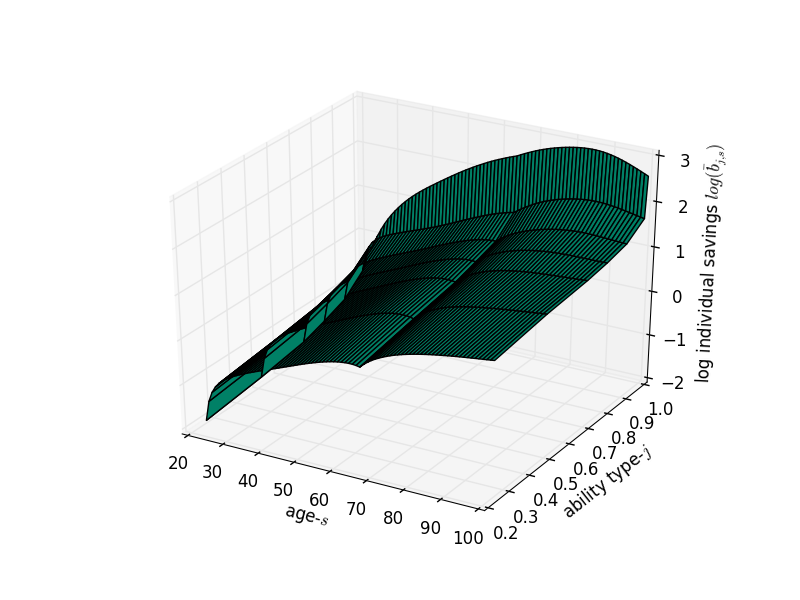
\includegraphics{images/SavSS_log.png}}}
%    \end{figure}
%
%    \begin{figure}[htb]\centering \captionsetup{width=4.0in}
%      \caption{\label{FigLabSS}\textbf{Stationary steady-state distribution of individual labor supply $\bar{n}_{j,s}$ for $S=80$ and $J=7$}}
%      \fbox{\resizebox{4.0in}{3.0in}{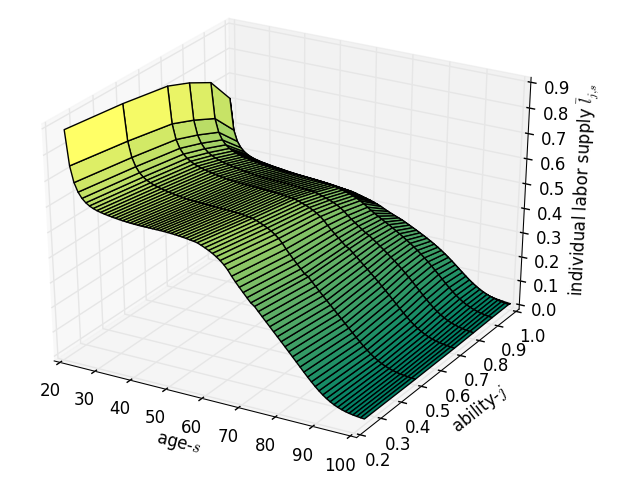
\includegraphics{images/LabSS.png}}}
%    \end{figure}
%
%    \begin{figure}[htb]\centering \captionsetup{width=4.0in}
%      \caption{\label{FigLogConsSS}\textbf{Stationary steady-state distribution of consumption $\bar{c}_{j,s}$ for $S=80$ and $J=7$}}
%      \fbox{\resizebox{4.0in}{3.0in}{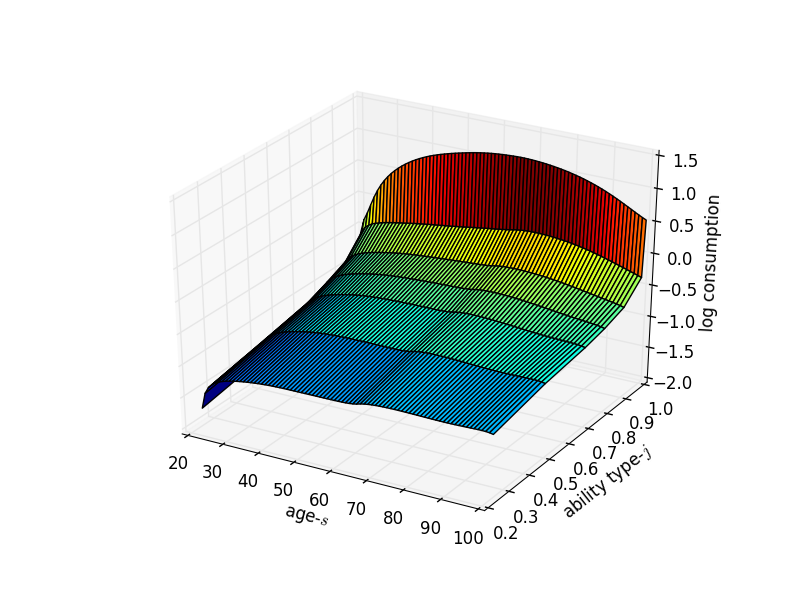
\includegraphics{images/ConsSS_log.png}}}
%    \end{figure}
%
%    Figure \ref{FigLogSavSS} shows the stationary steady-state distribution of individual savings $\bar{b}_{j,s}$ in logarithms, Figure \ref{FigLabSS} shows the stationary steady-state distribution of individual labor supply $\bar{n}_{j,s}$, and Figure \ref{FigLogConsSS} shows the steady-state distribution of consumption $\bar{c}_{j,s}$ in logarithms for a particular calibration of the model described in Table \ref{TabExogVars}. Notice from Figure \ref{FigLogConsSS} the hump-shaped pattern of consumption over the life cycle for each ability type, which is consistent with consumption data. Also note from the comparison of the distribution of savings in Figure \ref{FigLogSavSS} in comparison to the distribution of consumption in \ref{FigLogConsSS} that households use savings to smooth out consumption as much as possible, with a sharpe change in savings around retirement $s=R$ and only a small smooth lump in consumption at that age.

    The definition of the stationary non-steady-state equilibrium is similar to Definition \ref{DefEquilSS}, with the stationary steady-state equilibrium definition being a special case of the stationary non-steady-state equilibrium.

\ \\ 
WHAT FOLLOWS NEEDS UPDATING TO INCLUDE RICHER FIRM AND GOV'T, BUT IS HELPFUL IN SEEING THAT NON-SS EQ'M WILL LOOK LIKE...

\ \\

    \hrule
    \begin{definition}[\textbf{Stationary non-steady-state equilibrium}]\label{DefEquilNonSS}
      A non-autarkic stationary non-steady-state equilibrium in the overlapping generations model with $S$-period lived agents and heterogeneous ability $e_{j,s}$ is defined as allocations $n_{j,s,t}$ and $\hat{b}_{j,s+1,t+1}$ and prices $\hat{w}_t$ and $r_t$ for all $j$, $s$, and $t$ such that the following conditions hold:
       \begin{enumerate}
          \item households have symmetric beliefs $\Omega(\cdot)$ about the evolution of the distribution of savings, and those beliefs about the future distribution of savings equal the realized outcome (rational expectations),
            \begin{equation*}
              \bm{\hat{\Gamma}}_{t+u} = \bm{\hat{\Gamma}}^e_{t+u} = \Omega^u\left( \bm{\hat{\Gamma}}_t\right) \quad\forall t, \quad u\geq 1
            \end{equation*}
          \item households optimize according to \eqref{EqEulerLabStat}, \eqref{EqEulerSavStat}, and \eqref{EqEulerSavEpSstat}
          \item firms optimize according to \eqref{EqFOCwageStat} and \eqref{EqFOCrate}, and
          \item markets clear according to \eqref{EqMktClrLabStat} and \eqref{EqMktClrCapStat}.
       \end{enumerate}
    \end{definition}
    \hrule
   
   \ \\
   
    \noindent Taken together, the household labor-leisure and intended bequest decisions in the last period of life show that the optimal labor supply and optimal intended bequests for age $s=E+S$ are each functions of individual holdings of savings, total bequests received, and the prices in that period $n_{j,E+S,t}=\phi\bigl(\hat{b}_{j,E+S,t},\hat{BQ}_{j,t},\hat{w}_t,r_t\bigr)$ and $\hat{b}_{j,E+S+1,t+1}=\psi\bigl(\hat{b}_{j,E+S,t},\hat{BQ}_{j,t},\hat{w}_t,r_t\bigr)$. These two decisions are characterized by final-age version of the static labor supply Euler equation \eqref{EqEulerLabStat} and the static intended bequests Euler equation \eqref{EqEulerSavEpSstat}. Households in their second-to-last period of life in period $t$ have four decisions to make. They must choose how much to work this period $n_{j,E+S-1,t}$ and next period $n_{j,E+S,t+1}$, how much to save this period for next period $\hat{b}_{j,E+S,t+1}$, and how much to bequeath next period $\hat{b}_{j,E+S+1,t+2}$. The optimal responses for this individual are characterized by the $s=E+S-1$ and $s=E+S$ versions of the static Euler equations \eqref{EqEulerLabStat}, the $s=E+S-1$ version of the intertemporal Euler equation \eqref{EqEulerSavStat}, and the $s=E+S$ static bequest Euler equation \eqref{EqEulerSavEpSstat}, respectively.

    Optimal savings in the second-to-last period of life $s=E+S-1$ is a function of the current savings as well as the total bequests received and prices in the current period and in the next period $\hat{b}_{j,E+S,t+1} = \psi\bigl(\hat{b}_{j,E+S-1,t},\hat{BQ}_{j,t},\hat{w}_t,r_t,\hat{BQ}_{j,t+1},\hat{w}_{t+1},r_{t+1}|\Omega\bigr)$ given beliefs $\Omega$. As before, the optimal labor supply at age $s=E+S$ is a function of the next period's savings, bequests received, and prices $n_{j,E+S,t+1}=\phi\bigl(\hat{b}_{j,E+S,t+1},\hat{BQ}_{j,t+1},\hat{w}_{t+1},r_{t+1}\bigr)$. But the optimal labor supply at age $s=E+S-1$ is a function of the current savings, current bequests received, and the current prices as well as the future bequests received and future prices because of the dependence on the savings decision in that same period $n_{j,E+S-1,t}=\phi\bigl(\hat{b}_{j,E+S-1,t},\hat{BQ}_{j,t},\hat{w}_t,r_t,\hat{BQ}_{j,t+1},\hat{w}_{t+1},r_{t+1}|\Omega\bigr)$ given beliefs $\Omega$. By induction, we can show that the optimal labor supply, savings, and intended bequests functions for any individual with ability $j$, age $s$, and in period $t$ is a function of current holdings of savings and the lifetime path of total bequests received and prices given beliefs $\Omega$.
    \begin{align}
      n_{j,s,t} &= \phi\Bigl(\hat{b}_{j,s,t},\bigl(\hat{BQ}_{j,v},\hat{w}_v,r_v\bigr)_{v=t}^{t+S-s}|\Omega\Bigr) \quad\forall j,s,t \label{EqLabPolFuncGen} \\
      \hat{b}_{j,s+1,t+1} &= \psi\Bigl(\hat{b}_{j,s,t},\bigl(\hat{BQ}_{j,v},\hat{w}_v,r_v\bigr)_{v=t}^{t+S-s}|\Omega\Bigr) \quad\forall j,t \quad\text{and}\quad E+1\leq s\leq E+S \label{EqSavPolFuncGen}
    \end{align}

    If one knows the current distribution of households savings and intended bequests $\bm{\hat{\Gamma}}_t$ and has a beliefs function that predicts the law of motion over time for $\bm{\hat{\Gamma}}_t$, then one can predict time series for total bequests received $\hat{BQ}_{j,t}$, real wages $\hat{w}_t$ and real interest rates $r_t$ necessary for solving each household's optimal decisions. Characteristic (i) in equilibrium definition \ref{DefEquilNonSS} that individuals be able to forecast prices with perfect foresight over their lifetimes implies that each individual has correct information and beliefs about all the other individuals optimization problems and information. It also implies that the equilibrium allocations and prices are really just functions of the entire distribution of savings at a particular period, as well as a law of motion for that distribution of savings.

    In equilibrium, the steady-state household labor supplies $\bar{n}_{j,s}$ for all $j$ and $s$, the steady-state savings $\bar{b}_{j,E+S+1}$, the steady-state real wage $\bar{w}$, and the steady-state real rental rate $\bar{r}$ are simply functions of the steady-state distribution of savings $\bar{\Gamma}$. This is clear from the steady-state version of the capital market clearing condition \eqref{EqMktClrCapStat} and the fact that aggregate labor supply is a function of the sum of exogenous efficiency units of labor in the labor market clearing condition \eqref{EqMktClrLabStat}. And the two firm first order conditions for the real wage $\hat{w}_t$ \eqref{EqFOCwageStat} and real rental rate $r_t$ \eqref{EqFOCrate} are only functions of the stationary aggregate capital stock $\hat{K}_t$ and aggregate labor $\hat{L}_t$.

    \begin{figure}[htb]\centering \captionsetup{width=4.0in}
      \caption{\label{FigKpathTPI}\textbf{Equilibrium time path of $K_t$ for $S=80$ and $J=7$}}
      \fbox{\resizebox{4.0in}{3.0in}{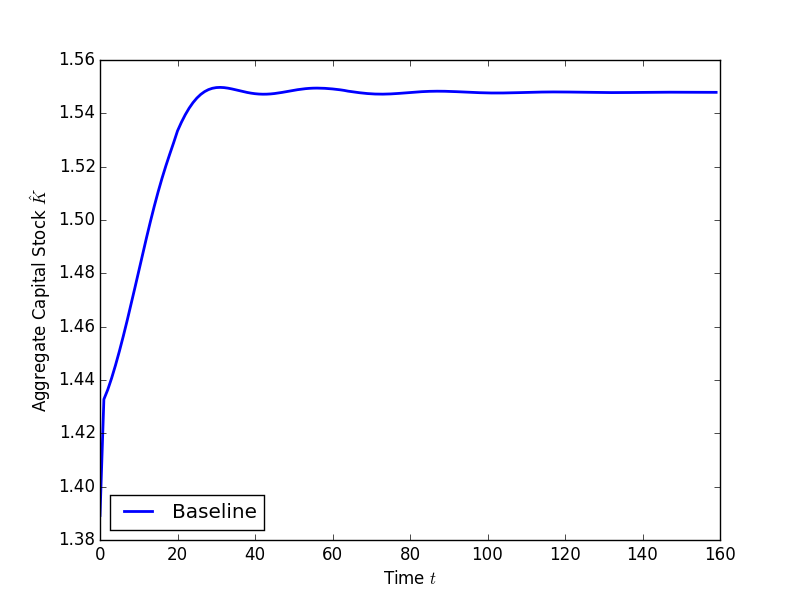
\includegraphics{images/KpathTPI.png}}}
    \end{figure}

    \begin{figure}[htb]\centering \captionsetup{width=4.0in}
      \caption{\label{FigLpathTPI}\textbf{Equilibrium time path of $L_t$ for $S=80$ and $J=7$}}
      \fbox{\resizebox{4.0in}{3.0in}{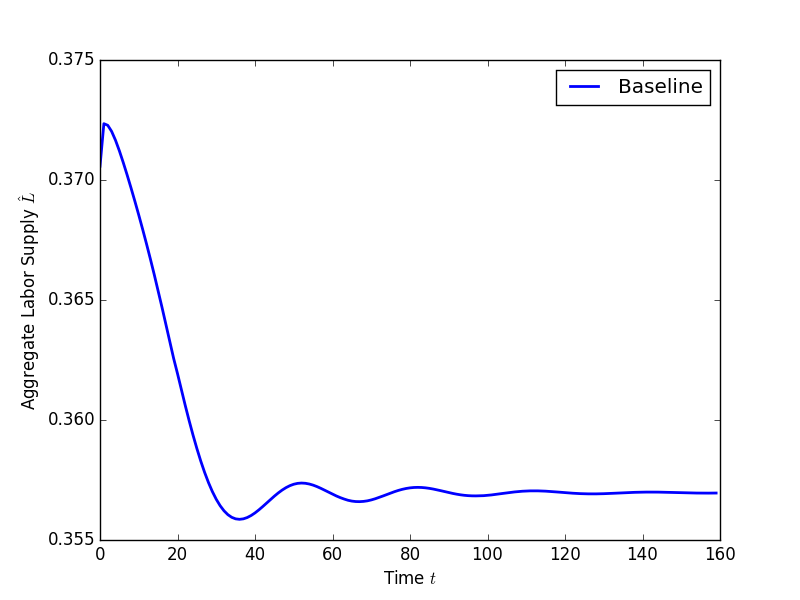
\includegraphics{images/LpathTPI.png}}}
    \end{figure}



\chapter{Numerical Solution}
\index{Numerical Solution%
@\emph{Numerical Solution}}%



%\pagestyle{empty}


FIRMS STUFF:
\section{Solving the model}

We'll solve the model in two steps.  First, we solve for the steady state prices and allocations.  Next, we iterate backwards solving for prices and allocations along the transition path to the steady state.

\subsection{Solving for the steady state}

On the supply side (with one sector), we have to solve for the factor prices, $\bar{i}$ and $bar{w}$ (the price of output $\bar{p}^{C}$ is normalized to one), the shadow price of capital, $\bar{q}^{C}$, and the allocations $\bar{EL}^{C}$, $\bar{K}^{C}$, $\bar{I}^{C}$.  From these all the other variables follow trivially.  

Start by solving for the steady-states of Equations \ref{eqn:opt_i} and \ref{eqn:foc_k}.  Equation \ref{eqn:opt_i} becomes:

\begin{equation}
\label{eqn:opt_i_ss}
\bar{q}^{C}=\underbrace{1-b^{C}-\bar{\Omega}^{C}\bar{\tau}^{b}(f_{e}-f_{b}b^{C})-f_{d}(1-f_{e})\bar{Z}^{C}}_{\text{function of only parameters}}
\end{equation}

This yields the solution to $\bar{q}^{C}$.

Next, consider the steady-state of Equation \ref{eqn:foc_k}:

\begin{equation}
\label{eqn:foc_k_ss}
\bar{q}^{C}=\frac{1}{1+\bar{\theta}}\left[(1-\delta^{C})\bar{q}^{C} + \frac{\partial \bar{X}^{C}}{\partial \bar{K}^{C}} - \{(1-\bar{\tau}^{b})\bar{\Omega}^{C}\bar{\tau}^{pC} + (1-f_{i}\bar{\tau}^{i})\bar{i}\bar{\Omega}^{C}b^{C} - \delta^{C}(1-b^{C}-\bar{\Omega}^{C}(1-f_{p}\bar{\tau}^{b}b^{C}))\}\right]
\end{equation}

We can rearrange this and solve for the steady-state marginal product of capital in sector $C$:

\begin{equation}
\label{eqn:mpk_ss}
\frac{\partial \bar{X}^{C}}{\partial \bar{K}^{C}} = (\bar{\theta}+\delta^{C})\bar{q}^{C} + (1-\bar{\tau}^{b})\bar{\Omega}^{C}\bar{\tau}^{pC} + (1-f_{i}\bar{\tau}^{i})\bar{i}\bar{\Omega}^{C}b^{C} - \delta^{C}(1-b^{C}-\bar{\Omega}^{C}(1-f_{p}\bar{\tau}^{b}b^{C}))
\end{equation}

Notice that given Equation \ref{eqn:opt_i_ss}, the RHS to the above equation is function of parameters and the steady state nominal interest rate, $\bar{i}$.  The LHS of the equation is a function of $\bar{K}^{C}$ and $\bar{EL}^{C}$.

I think we can use the following to identify the SS values of the variables of interest:
\begin{enumerate}
\item $\bar{i}$ will be determined by the SS of the household's Euler equations (I think this can be done as described in the HH sol'n method)
\item $\bar{w}$ will be determined by the SS of the household's FOCs for labor supply ((I think this can be done as described in the HH sol'n method)
\item $\bar{q}^{C}$ is determined by Equation \ref{eqn:opt_i_ss}
\item $\bar{EL}^{C}$ is determined by the SS version of Equation \ref{eqn:foc_l}, plus $\bar{w}$
\item $\bar{K}^{C}$ is determined by Equation \ref{eqn:mpk_ss} and $\bar{i}$
\item $\bar{I}^{C}$ is then solved for using the steady state law of motion for capital $\implies \bar{I}^{C}=\delta^{C}\bar{K}^{C}$
\end{enumerate}

In solving for $\bar{EL}^{C}$ and $\bar{K}^{C}$, note that we'll have use the MPK and the MPL simultaneously.  Given our production function, we have:

\begin{equation}
\label{eqn:mpk}
\frac{\partial X^{C}_{u}}{\partial K^{C}_{u}} = \left[(\gamma_{C})^{1/\epsilon_{C}}(K^{C}_{u})^{(\epsilon_{C}-1)/\epsilon_{C}}+(1-\gamma_{C})^{1/\epsilon_{C}}(EL^{C}_{u})^{(\epsilon_{C}-1)/\epsilon_{C}}\right]^{1/(\epsilon_{C}-1)}(\gamma_{C})^{1/\epsilon_{C}}(K^{C}_{u})^{-1/\epsilon_{C}}
\end{equation}

and 

\begin{equation}
\label{eqn:mpl}
\frac{\partial X^{C}_{u}}{\partial EL^{C}_{u}} = \left[(\gamma_{C})^{1/\epsilon_{C}}(K^{C}_{u})^{(\epsilon_{C}-1)/\epsilon_{C}}+(1-\gamma_{C})^{1/\epsilon_{C}}(EL^{C}_{u})^{(\epsilon_{C}-1)/\epsilon_{C}}\right]^{1/(\epsilon_{C}-1)}(1-\gamma_{C})^{1/\epsilon_{C}}(EL^{C}_{u})^{-1/\epsilon_{C}}
\end{equation}

We know that, at an optimum, the marginal revenue product of labor equals the wage rate, and the marginal revenue product of capital equals a function of the interest rate, marginal $q$, and the model parameters.  Call this function $g(i_{u},q^{C}_{u},q^{C}_{u-1},\Theta)$.  We thus have $p^{C}_{u}\frac{\partial X^{C}_{u}}{\partial EL^{C}_{u}} =w_{u}$ and $p^{C}_{u}\frac{\partial X^{C}_{u}}{\partial K^{C}_{u}}=g(i_{u},q^{C}_{u},q^{C}_{u-1},\Theta)$.  Dividing these two equations, we have:

\begin{equation}
\label{eqn:cap_lab_ratio}
\begin{split}
& \frac{\frac{\partial X^{C}_{u}}{\partial K^{C}_{u}}}{\frac{\partial X^{C}_{u}}{\partial EL^{C}_{u}}} =\frac{(\gamma_{C})^{1/\epsilon_{C}}(K^{C}_{u})^{-1/\epsilon_{C}}}{(1-\gamma_{C})^{1/\epsilon_{C}}(EL^{C}_{u})^{-1/\epsilon_{C}}}-=\frac{g(i_{u},q^{C}_{u},q^{C}_{u-1},\Theta)}{w_{u}} \\
& \implies \frac{K^{C}_{u}}{EL^{C}_{u}} =\frac{(1-\gamma_{C})}{\gamma_{C}}\left(\frac{w_{u}} {g(i_{u},q^{C}_{u},q^{C}_{u-1},\Theta)}\right)^{\epsilon_{C}} \\
\end{split}
\end{equation}

We can use the SS version of Equation \ref{eqn:cap_lab_ratio} to solve for capital as function of labor (and $\bar{q}, \bar{i}, \bar{w}$), and then use that in the SS version of Equation \ref{eqn:mpl} to solve for labor as s function of $\bar{q}, \bar{i}, \bar{w}$.  We then go back to the SS version of Equation \ref{eqn:cap_lab_ratio} to get the SS choice of capital as a function of $\bar{q}, \bar{i}, \bar{w}$.

All of the above will work for each sector in a model with any number of sectors (though care has to be taken to include the prices of output and capital in those other sectors, since only one sector's output can be the numeraire).

\subsection{Solving for the transition path}

I believe we can just use the Euler equations to go backwards in time, from the SS back along the transition path to $t=0$.  Assume period $T$ is the SS,  The solution would look like the following:

\begin{enumerate}
\item Use Equation \ref{eqn:foc_k} to solve for the for $q^{C}_{T-1}$ since we have the solution to the RHS of the equation after we've solved for the SS.
\item Use the law of motion for capital to find: $K^{C}_{T-1}=\frac{K^{C}_{T}-I^{C}_{T-1}}{(1-\delta^{C})}=\frac{\bar{K}^{C}-I^{C}_{T-1}}{(1-\delta^{C})}$
\item Use Equation \ref{eqn:opt_i} and the value of $q^{C}_{T-1}$ to find $I^{C}_{T-1}$ (and $K^{C}_{T-1}$ given the law of motion relationship.
\item Given $w_{T-1}$ we can use the FOC for labor demand to find $EL^{C}_{T-1}$
\item Given $i_{T-1}$ we can use Equation \ref{eqn:foc_k} to solve for $q^{C}_{T-2}$ 
\item We then repeat the above steps until we work back to $t=0$.
\end{enumerate}



To solve for any stationary non-steady-state equilibrium time path of the economy from an arbitrary current state to the steady state, we follow the time path iteration (TPI) method of \citet{AuerbachKotlikoff:1987}. Appendix \ref{AppNonSSsolve} details how to solve for the non-steady-state equilibrium time path using the TPI method. The approach is to choose an arbitrary time path for the stationary aggregate capital stock $\hat{K}_t$, stationary aggregate labor $\hat{L}_t$, and total bequests received $\hat{BQ}_{j,t}$ for each type $j$. This initial guess of a path implies arbitrary beliefs that violate the rational expectations requirement. We then solve for households' optimal decisions given the time paths of those variables, which decisions imply new time paths of those variables. We then update the time path as a convex combination of the initial guess and the new implied path. Figure \ref{FigKpathTPI} shows the equilibrium time path of the aggregate capital stock for the calibration described in Table \ref{TabExogVars} for $T=160$ periods starting from an initial distribution of savings in which $b_{j,s,1}=\bm{\bar{\Gamma}}$ for all $j$ and $s$ in the case that no policy experiment takes place. The initial capital stock $\hat{K}_1$ is not at the steady state $\bar{K}$ because the initial population distribution is not at the steady-state.

\section{Solving for stationary steady-state equilibrium}\label{AppSSsolve}

  \setcounter{equation}{0}
  \renewcommand\theenumi{\arabic{enumi}}
  \renewcommand\theenumii{\alph{enumii}}
  \renewcommand\theenumiii{\roman{enumiii}}

  This section describes the solution method for the stationary steady-state equilibrium described in Definition \ref{DefEquilSS}.
  
  
  We can try to draw some nice tree structures as in \citet{FR1993}, but here's how the consumer side of the problem is solved;
\begin{enumerate}
\item The firm's problem determines prices of output from each sector and industry in a given year: $p_{m,t,C}$ and $p_{m,t,NC}$.
\item Given these, Equation \ref{eqn:price_comp} determines $p_{m,t}$, the price of composite output for sector $m$.
\item The price of composite output in each sector $m$ is related to the prices of the $I$ consumption goods through the matrix $Z$ as described in Equation \ref{eqn:mix_cons_price}.
\item Equation \ref{eqn:composite_price} describes how the composite consumption good price is determined from these individual consumption good prices, for each age $s$ composite consumption bundle.
\item With all prices in hand, we can solve for quantities demanded.  Using $p_{s,t}$ and $p_{i,t}$ in Equation \ref{EqBC}, we can then solve the consumers problem for the choice of $\tilde{c}_{j,s,t}$. 
\item These $\tilde{c}_{j,s,t}$ then determine demand for each individual consumption good, $c_{i,j,s,t}$ by Equation \ref{eqn:cons_solve}.
\item Demands for consumption goods are then translated into demands for output from each industry $m$ by Equation \ref{eqn:mix_cons}.
\item Demand for output from each sector (corporate or non-corporate) in industry $m$ are then determined by Equations \ref{eqn:demand_XmtC} and \ref{eqn:demand_XmtNC}.
\item These demands are then checked against the supply determined in (1).  If they match, we've found an eq'm. If not, we update the guess of $r$, $w$, $BQ$ and work from (1)-(8) again.
\end{enumerate}

  \begin{enumerate}
    \item Use the techniques in Appendix \ref{AppPopGrowth} to solve for the steady-state population distribution vector $\bm{\bar{\omega}}$ of the exogenous population process.
    \item Choose an initial guess for the stationary steady-state distribution of capital $\bar{b}_{j,s+1}$ for all $j$ and $s=E+2,E+3,...E+S+1$ and labor supply $\bar{n}_{j,s}$ for all $j$ and $s$.
      \begin{itemize}
        \item A good first guess is a large positive number for all the $\bar{n}_{j,s}$ that is slightly less than $\tilde{l}$ and to choose some small positive number for $\bar{b}_{j,s+1}$ that is small enough to be less than the minimum income that an individual might have $\bar{w}e_{j,s}\bar{n}_{j,s}$.
      \end{itemize}
    \item Perform an unconstrained root finder that chooses $\bar{n}_{j,s}$ and $\bar{b}_{j,s+1}$ that solves the $2JS$ stationary steady-state Euler equations.
    \item Make sure none of the implied steady-state consumptions $\bar{c}_{j,s}$ is less-than-or-equal-to zero.
      \begin{itemize}
        \item If one consumption is less-than-or-equal-to zero $\bar{c}_{j,s}\leq 0$, then try different starting values.
      \end{itemize}
    \item Make sure that none of the Euler errors is too large in absolute value for interior stationary steady-state values. A steady-state Euler error is the following, which is supposed to be close to zero for all $j$ and $s$:
      \begin{align}
        \begin{split}
          &\frac{\chi^n_{s}\left(\frac{b}{\tilde{l}}\right)\left(\frac{\bar{n}_{j,s}}{\tilde{l}}\right)^{v-1}\left[1 - \left(\frac{\bar{n}_{j,s}}{\tilde{l}}\right)\right]^{\frac{1-v}{v}}}{(\bar{c}_{j,s})^{-\sigma}\left(\bar{w} e_{j,s} - \frac{\partial\bar{T}_{j,s}}{\partial \bar{n}_{j,s}}\right)} - 1 \\
          &\qquad\qquad\qquad\qquad\qquad\qquad\qquad\forall j\quad\text{and}\quad E+1\leq s\leq E+S
        \end{split} \label{EqSSeulerrLab} \\
        \begin{split}
          &\frac{e^{-g_y\sigma}\left(\rho_s\chi^b \left(\bar{b}_{j,s+1}\right)^{-\sigma} + \beta(1-\rho_s)(\bar{c}_{j,s+1})^{-\sigma}\left[(1 + \bar{r}) - \frac{\partial \bar{T}_{j,s+1}}{\partial \bar{b}_{j,s+1}}\right]\right)}{(\bar{c}_{j,s})^{-\sigma}} - 1 \\
          &\qquad\qquad\qquad\qquad\qquad\qquad\qquad\forall j \quad\text{and}\quad E+1\leq s\leq E+S-1 \\
        \end{split} \label{EqSSeulerrSav} \\
        &\frac{\chi^b e^{-g_y\sigma}(\bar{b}_{j,E+S+1})^{-\sigma}}{\left(\bar{c}_{j,E+S}\right)^{-\sigma}} - 1 \quad\forall j \label{EqSSeulerrBeq}
      \end{align}
  \end{enumerate}


\newpage
\section{Solving for stationary non-steady-state equilibrium by time path iteration}\label{AppNonSSsolve}

  \setcounter{equation}{0}

  This section outlines the benchmark time path iteration (TPI) method of \citet{AuerbachKotlikoff:1987} for solving the stationary non-steady-state equilibrium transition path of the distribution of savings. TPI finds a fixed point for the transition path of the distribution of capital for a given initial state of the distribution of capital. The idea is that the economy is infinitely lived, even though the agents that make up the economy are not. Rather than recursively solving for equilibrium policy functions by iterating on individual value functions, one must recursively solve for the policy functions by iterating on the entire transition path of the endogenous objects in the economy (see \citet[ch. 17]{StokeyLucas:1989}).

  The key assumption is that the economy will reach the steady-state equilibrium described in Definition \ref{DefEquilSS} in a finite number of periods $T<\infty$ regardless of the initial state. Let $\bm{\hat{\Gamma}}_t$ represent the distribution of stationary savings at time $t$.
  \begin{equation}\tag{\ref{EqSavDist}}
    \bm{\hat{\Gamma}}_t \equiv \Bigl\{\bigl\{\hat{b}_{j,s,t}\bigr\}_{j=1}^J\Bigr\}_{s=E+2}^{E+S+1}, \quad\forall t
  \end{equation}
  In Section \ref{SecMCEqlbm}, we describe how the stationary non-steady-state equilibrium time path of allocations and price is described by functions of the state $\bm{\hat{\Gamma}}_t$ and its law of motion. TPI starts the economy at any initial distribution of savings $\bm{\hat{\Gamma}}_1$ and solves for its equilibrium time path over $T$ periods to the steady-state distribution $\bm{\bar{\Gamma}}_T$.

  The first step is to assume an initial transition path for aggregate stationary capital $\bm{\hat{K}}^i = \left\{\hat{K}_1^i,\hat{K}_2^i,...\hat{K}_T^i\right\}$, aggregate stationary labor $\bm{\hat{L}}^i = \left\{\hat{L}_1^i,\hat{L}_2^i,...\hat{L}_T^i\right\}$, and total bequests received $\bm{\hat{BQ}}_j^i=\{\hat{BQ}_{j,1}^i,\hat{BQ}_{j,2}^i,...\hat{BQ}_{j,T}^i\}$ for each ability type $j$ such that $T$ is sufficiently large to ensure that $\bm{\hat{\Gamma}}_T = \bar{\bm{\Gamma}}$, $\hat{K}_T^i\left(\bm{\Gamma}_T\right)$, $\hat{L}_T^i\left(\bm{\Gamma}_T\right) = \bar{L}\left(\bar{\bm{\Gamma}}\right)$, and $\hat{BQ}_{j,T}^i\left(\bm{\Gamma}_T\right) = \bar{BQ}_j\left(\bar{\bm{\Gamma}}\right)$ for all $t\geq T$. The superscript $i$ is an index for the iteration number. The transition paths for aggregate capital and aggregate labor determine the transition paths for both the real wage $\bm{\hat{w}}^i = \left\{\hat{w}_1^i,\hat{w}_2^i,...\hat{w}_T^i\right\}$ and the real return on investment $\bm{r}^i = \left\{r_1^i,r_2^i,...r_T^i\right\}$. The time paths for the total bequests received also figure in each period's budget constraint and are determined by the distribution of savings and intended bequests.

  The exact initial distribution of capital in the first period $\bm{\hat{\Gamma}}_1$ can be arbitrarily chosen as long as it satisfies the stationary capital market clearing condition \eqref{EqMktClrCapStat}.
  \begin{equation}\label{EqMktClrCapStat1}
    \hat{K}_1 = \frac{1}{1 + \tilde{g}_{n,1}}\sum_{s=E+2}^{E+S+1}\sum_{j=1}^{J}\hat{\omega}_{s-1,0}\lambda_j \hat{b}_{j,s,1}
  \end{equation}
  Simiilarly, each initial value of total bequests received $\hat{BQ}_{j,1}^i$ must be consistent with the initial distribution of capital through the stationary version of \eqref{EqTotBeq}.
  \begin{equation}\label{EqTotBeqStat1}
    \hat{BQ}_{j,1} = \frac{(1+r_1)\lambda_j}{1+\tilde{g}_{n,1}}\sum_{s=E+1}^{E+S}\rho_s\hat{\omega}_{s,0}\hat{b}_{j,s+1,1} \quad\forall j
  \end{equation}
  However, this is not the case with $\hat{L}_1^i$. Its value will be endogenously determined in the same way the $K_2^i$ is. For this reason, a logical initial guess for the time path of aggregate labor is the steady state in every period $L_t^1 = \bar{L}$ for all $1\leq t\leq T$.

  It is easiest to first choose the initial distribution of savings $\bm{\hat{\Gamma}}_1$ and then choose an initial aggregate capital stock $\hat{K}_1^i$ and initial total bequests received $\hat{BQ}_{j,1}^i$ that correspond to that distribution. As mentioned earlier, the only other restrictions on the initial transition paths for aggregate capital, aggregate labor, and total bequests received is that they equal their steady-state levels $\hat{K}_T^i = \bar{K}\left(\bm{\bar{\Gamma}}\right)$, $\hat{L}_T^i = \bar{L}\left(\bm{\bar{\Gamma}}\right)$, and $\hat{BQ}_{j,T}^i = \bar{BQ}_j\left(\bm{\bar{\Gamma}}\right)$ by period $T$. \citet{EvansPhillips:2014} have shown that the initial guess for the aggregate capital stocks $\hat{K}_t^i$ for periods $1<t<T$ can take on almost any positive values satisfying the constraints above and still have the time path iteration converge.

  Given the initial savings distribution $\bm{\hat{\Gamma}}_1$ and the transition paths of aggregate capital $\bm{\hat{K}}^i = \left\{\hat{K}_1^i,\hat{K}_2^i,...\hat{K}_T^i\right\}$, aggregate labor $\bm{\hat{L}}^i = \left\{\hat{L}_1^i,\hat{L}_2^i,...\hat{L}_T^i\right\}$, and total bequests received $\bm{\hat{BQ}}_j^i = \left\{\hat{BQ}_{j,1}^i,\hat{BQ}_{j,2}^i,...\hat{BQ}_{j,T}^i\right\}$, as well as the resulting real wage $\bm{\hat{w}}^i = \left\{\hat{w}_1^i,\hat{w}_2^i,...\hat{w}_T^i\right\}$, and real return to savings $\bm{r}^i = \left\{r_1^i,r_2^i,...r_T^i\right\}$, one can solve for the period-1 optimal labor supply and intended bequests for each type $j$ of $s=E+S$-aged agents in the last period of their lives $n_{j,E+S,1}=\phi_{j,E+S}(\hat{b}_{j,E+S,1},\hat{BQ}_{j,E+S,1},\hat{w}_1,r_1)$ and $\hat{b}_{j,E+S+1,2}=\psi_{j,E+S}(\hat{b}_{j,E+S,1},\hat{BQ}_{j,E+S,1},\hat{w}_1,r_1)$ using his two $s=E+S$ static Euler equations \eqref{EqEulerLabStat} and \eqref{EqEulerSavEpSstat}.
  \begin{equation}\label{EqEulerSlabt1}
    \begin{split}
      &(\hat{c}_{j,E+S,1})^{-\sigma}\Biggl(\hat{w}_1^i e_{j,E+S} - \frac{\partial\hat{T}_{j,E+S,1}}{\partial n_{j,E+S,1}}\Biggr) = ... \\
      &\qquad\qquad\qquad\qquad \chi^n_{E+S}\biggl(\frac{b}{\tilde{l}}\biggr)\biggl(\frac{n_{j,E+S,1}}{\tilde{l}}\biggr)^{v-1}\Biggl[1 - \biggl(\frac{n_{j,E+S,1}}{\tilde{l}}\biggr)\Biggr]^{\frac{1-v}{v}} \quad\forall j \\
      &\quad\text{where}\quad \hat{c}_{j,E+S,1} = ... \\
      &\qquad\qquad\qquad \left(1 + r_1^i\right)\hat{b}_{j,E+S,1} + \hat{w}_1^i e_{j,E+S}n_{j,E+S,1} + \frac{\hat{BQ}_{j,1}}{\lambda_j} - e^{g_y}\hat{b}_{j,E+S+1,2} - \hat{T}_{j,E+S,1} \\
      &\quad\text{and}\quad \frac{\partial \hat{T}_{j,E+S,1}}{\partial n_{j,E+S,1}} = ... \\
      &\qquad\qquad\qquad \hat{w}_1^i e_{j,E+S}\biggl[\tau^I\bigl(F\hat{a}_{j,E+S,1}\bigr) + \frac{\hat{a}_{j,E+S,1}CDF\bigl[2A(F\hat{a}_{j,E+S,1})+B\bigr]}{\bigl[A(F\hat{a}_{j,E+S,1})^2+B(F \hat{a}_{j,E+S,1})+C\bigr]^2} + \tau^P\Biggr]
    \end{split}
  \end{equation}
  \begin{equation}\label{EqEulerSbeqt1}
    (\hat{c}_{j,E+S,1})^{-\sigma} = \chi^b e^{-g_y\sigma}(\hat{b}_{j,E+S+1,2})^{-\sigma} \quad\forall j
  \end{equation}
  Note that this is simply two equations \eqref{EqEulerSlabt1} and \eqref{EqEulerSbeqt1} and two unknowns $n_{j,E+S,1}$ and $\hat{b}_{j,E+S+1,2}$.

  We then solve the problem for all $j$ types of $E+S-1$-aged individuals in period $t=1$, each of which entails labor supply decisions in the current period $n_{j,E+S-1,1}$ and in the next period $n_{j,E+S,2}$, a savings decision in the current period for the next period $\hat{b}_{j,E+S,2}$ and an intended bequest decision in the last period $\hat{b}_{j,E+S+1,3}$. The labor supply decision in the initial period and the savings period in the initial period for the next period for each type $j$ of $E+S-1$-aged individuals are policy functions of the current savings and the total bequests received and prices in this period and the next $\hat{b}_{j,E+S,2} = \psi_{j,E+S-1}(\hat{b}_{j,E+S-1,1},\{\hat{BQ}_{j,t},\hat{w}_t,r_t\}_{t=1}^2)$ and $\hat{n}_{j,E+S-1,1} = \phi_{j,E+S-1}(\hat{b}_{j,E+S-1,1},\{\hat{BQ}_{j,t},\hat{w}_t,r_t\}_{t=1}^2)$. The labor supply and intended bequests decisions in the next period are simply functions of the savings, total bequests received, and prices in that period $\hat{n}_{j,E+S,2} = \phi_{j,E+S}(\hat{b}_{j,E+S,2},\hat{BQ}_{j,2},\hat{w}_2,r_2)$ and $\hat{b}_{j,E+S+1,3} = \psi_{j,E+S}(\hat{b}_{j,E+S,2},\hat{BQ}_{j,2},\hat{w}_2,r_2)$. These four functions are characterized by the following versions of equations \eqref{EqEulerLabStat}, \eqref{EqEulerSavStat}, and \eqref{EqEulerSavEpSstat}.
  \begin{equation}\label{EqEulerSm1labt1}
    \begin{split}
      &(\hat{c}_{j,E+S-1,1})^{-\sigma}\Biggl(\hat{w}_1^i e_{j,E+S-1} - \frac{\partial\hat{T}_{j,E+S-1,1}}{\partial n_{j,E+S-1,1}}\Biggr) = ... \\
      &\qquad\qquad\qquad \chi^n_{E+S-1}\biggl(\frac{b}{\tilde{l}}\biggr)\biggl(\frac{n_{j,E+S-1,1}}{\tilde{l}}\biggr)^{v-1}\Biggl[1 - \biggl(\frac{n_{j,E+S-1,1}}{\tilde{l}}\biggr)\Biggr]^{\frac{1-v}{v}} \quad\forall j
    \end{split}
  \end{equation}
  \begin{equation}\label{EqEulerSm1savt1}
    \begin{split}
      &(\hat{c}_{j,E+S-1,1})^{-\sigma} = ... \\
      &e^{-g_y\sigma}\Biggl(\rho_{E+S-1}\chi^b \bigl(\hat{b}_{j,E+S,2}\bigr)^{-\sigma} + \beta(1-\rho_{E+S-1})(\hat{c}_{j,E+S,2})^{-\sigma}\Biggl[(1 + r_2^i) - \frac{\partial T_{j,E+S,2}}{\partial b_{j,E+S,2}}\Biggr]\Biggr) \\
      &\qquad\qquad\qquad\qquad\qquad\qquad\qquad\qquad\qquad\qquad\qquad\qquad\qquad\qquad\qquad\qquad\forall j \\
      &\qquad\text{where}\quad \frac{\partial T_{j,E+S,2}}{\partial b_{j,E+S,2}} = ...\\
      &\qquad\qquad r_2^i\Biggl(\tau^I(F\hat{a}_{j,E+S,2}) + \frac{F\hat{a}_{j,E+S,2}CD\left[2A(F\hat{a}_{j,E+S,2}) + B\right]}{\left[A(F\hat{a}_{j,E+S,2})^2 + B(F\hat{a}_{j,E+S,2}) + C\right]^2}\Biggr) ... \\
      &\qquad\qquad \tau^W(\hat{b}_{j,E+S,2}) + \frac{\hat{b}_{j,E+S,2}PHM}{\left(H\hat{b}_{j,E+S,2} + M\right)^2}
    \end{split}
  \end{equation}
  \begin{equation}\label{EqEulerSlabt2}
    \begin{split}
      &(\hat{c}_{j,E+S,2})^{-\sigma}\Biggl(\hat{w}_2^i e_{j,E+S} - \frac{\partial\hat{T}_{j,E+S,2}}{\partial n_{j,E+S,2}}\Biggr) = ... \\
      &\qquad\qquad\qquad \chi^n_{E+S}\biggl(\frac{b}{\tilde{l}}\biggr)\biggl(\frac{n_{j,E+S,2}}{\tilde{l}}\biggr)^{v-1}\Biggl[1 - \biggl(\frac{n_{j,E+S,2}}{\tilde{l}}\biggr)\Biggr]^{\frac{1-v}{v}} \quad\forall j
    \end{split}
  \end{equation}
  \begin{equation}\label{EqEulerSsavt2}
    (\hat{c}_{j,E+S,2})^{-\sigma} = \chi^b e^{-g_y\sigma}(\hat{b}_{j,E+S+1,3})^{-\sigma} \quad\forall j
  \end{equation}
  Note that this is four equations \eqref{EqEulerSm1labt1}, \eqref{EqEulerSm1savt1}, \eqref{EqEulerSlabt2}, and \eqref{EqEulerSsavt2} and four unknowns $n_{j,E+S-1,1}$, $\hat{b}_{j,E+S,2}$, $n_{j,E+S,2}$, and $\hat{b}_{j,E+S+1,3}$.

  This process is repeated for every age of household alive in $t=1$ down to the age $s=E+1$ household at time $t=1$. Each of these households $j$ solves the full set of remaining $S-s+1$ labor supply decisions, $S-s$ savings decisions, and one intended bequest decision at the end of life. After the full set of lifetime decisions has been solved for all the households alive at time $t=1$, each ability $j$ household born in period $t\geq 2$ can be solved for, the solution to which is characterized by the following full set of Euler equations analogous to \eqref{EqEulerLabStat}, \eqref{EqEulerSavStat}, and \eqref{EqEulerSavEpSstat}.
  \begin{equation}\label{EqEulerslabt}
    \begin{split}
      &(\hat{c}_{j,s,t})^{-\sigma}\Biggl(\hat{w}_t^i e_{j,s} - \frac{\partial\hat{T}_{j,s,t}}{\partial n_{j,s,t}}\Biggr) =  \chi^n_{s}\biggl(\frac{b}{\tilde{l}}\biggr)\biggl(\frac{n_{j,s,t}}{\tilde{l}}\biggr)^{v-1}\Biggl[1 - \biggl(\frac{n_{j,s,t}}{\tilde{l}}\biggr)\Biggr]^{\frac{1-v}{v}} \\
      &\qquad\qquad\qquad\qquad\qquad\forall j \quad\text{and}\quad E+1\leq s\leq E+S\quad\text{and}\quad t\geq 2
    \end{split}
  \end{equation}

  \begin{equation}\label{EqEulersSavt}
    \begin{split}
      &(\hat{c}_{j,s,t})^{-\sigma} = ... \\
      &e^{-g_y\sigma}\Biggl(\rho_{s}\chi^b \bigl(\hat{b}_{j,s+1,t+1}\bigr)^{-\sigma} + \beta(1-\rho_{s})(\hat{c}_{j,s+1,t+1})^{-\sigma}\Biggl[(1 + r_{t+1}^i) - \frac{\partial T_{j,s+1,t+1}}{\partial b_{j,s+1,t+1}}\Biggr]\Biggr) \\
      &\qquad\qquad\qquad\forall j \quad\text{and}\quad E+1\leq s\leq E+S-1 \quad\text{and}\quad t\geq 2
    \end{split}
  \end{equation}

  \begin{equation}\label{EqEulerSsavt}
    (\hat{c}_{j,E+S,t})^{-\sigma} = \chi^b e^{-g_y\sigma}(\hat{b}_{j,E+S+1,t+1})^{-\sigma} \quad\forall j \quad\text{and}\quad t\geq 2
  \end{equation}
  For each household of ability type $j$ entering the economy in period $t\geq 1$, the entire set of $2S$ lifetime decisions is characterized by the $2S$ equations represented in \eqref{EqEulerslabt}, \eqref{EqEulersSavt}, and \eqref{EqEulerSsavt}.

  We can then solve for the entire lifetime of savings and labor supply decisions for each age $s=1$ individual in periods $t=2,3,...T$. The central part of the schematic diagram in Figure \ref{FigTPIdiag} shows how this process is done in order to solve for the equilibrium time path of the economy from period $t=1$ to $T$. Note that for each full lifetime savings and labor supply path solved for an individual born in period $t\geq 2$, we can solve for the aggregate capital stock and total bequests received implied by those savings decisions $\bm{\hat{K}}^{i'}$ and $\bm{\hat{BQ}}_{j}^{i'}$ and aggregate labor implied by those labor supply decisions $\bm{\hat{L}}^{i'}$.

  \begin{figure}[p]\centering \captionsetup{width=4.0in}
    \caption{\label{FigTPIdiag}\textbf{Diagram of TPI solution method within each iteration for $S=4$ and $J=1$}}
    \fbox{\resizebox{4.2in}{6.0in}{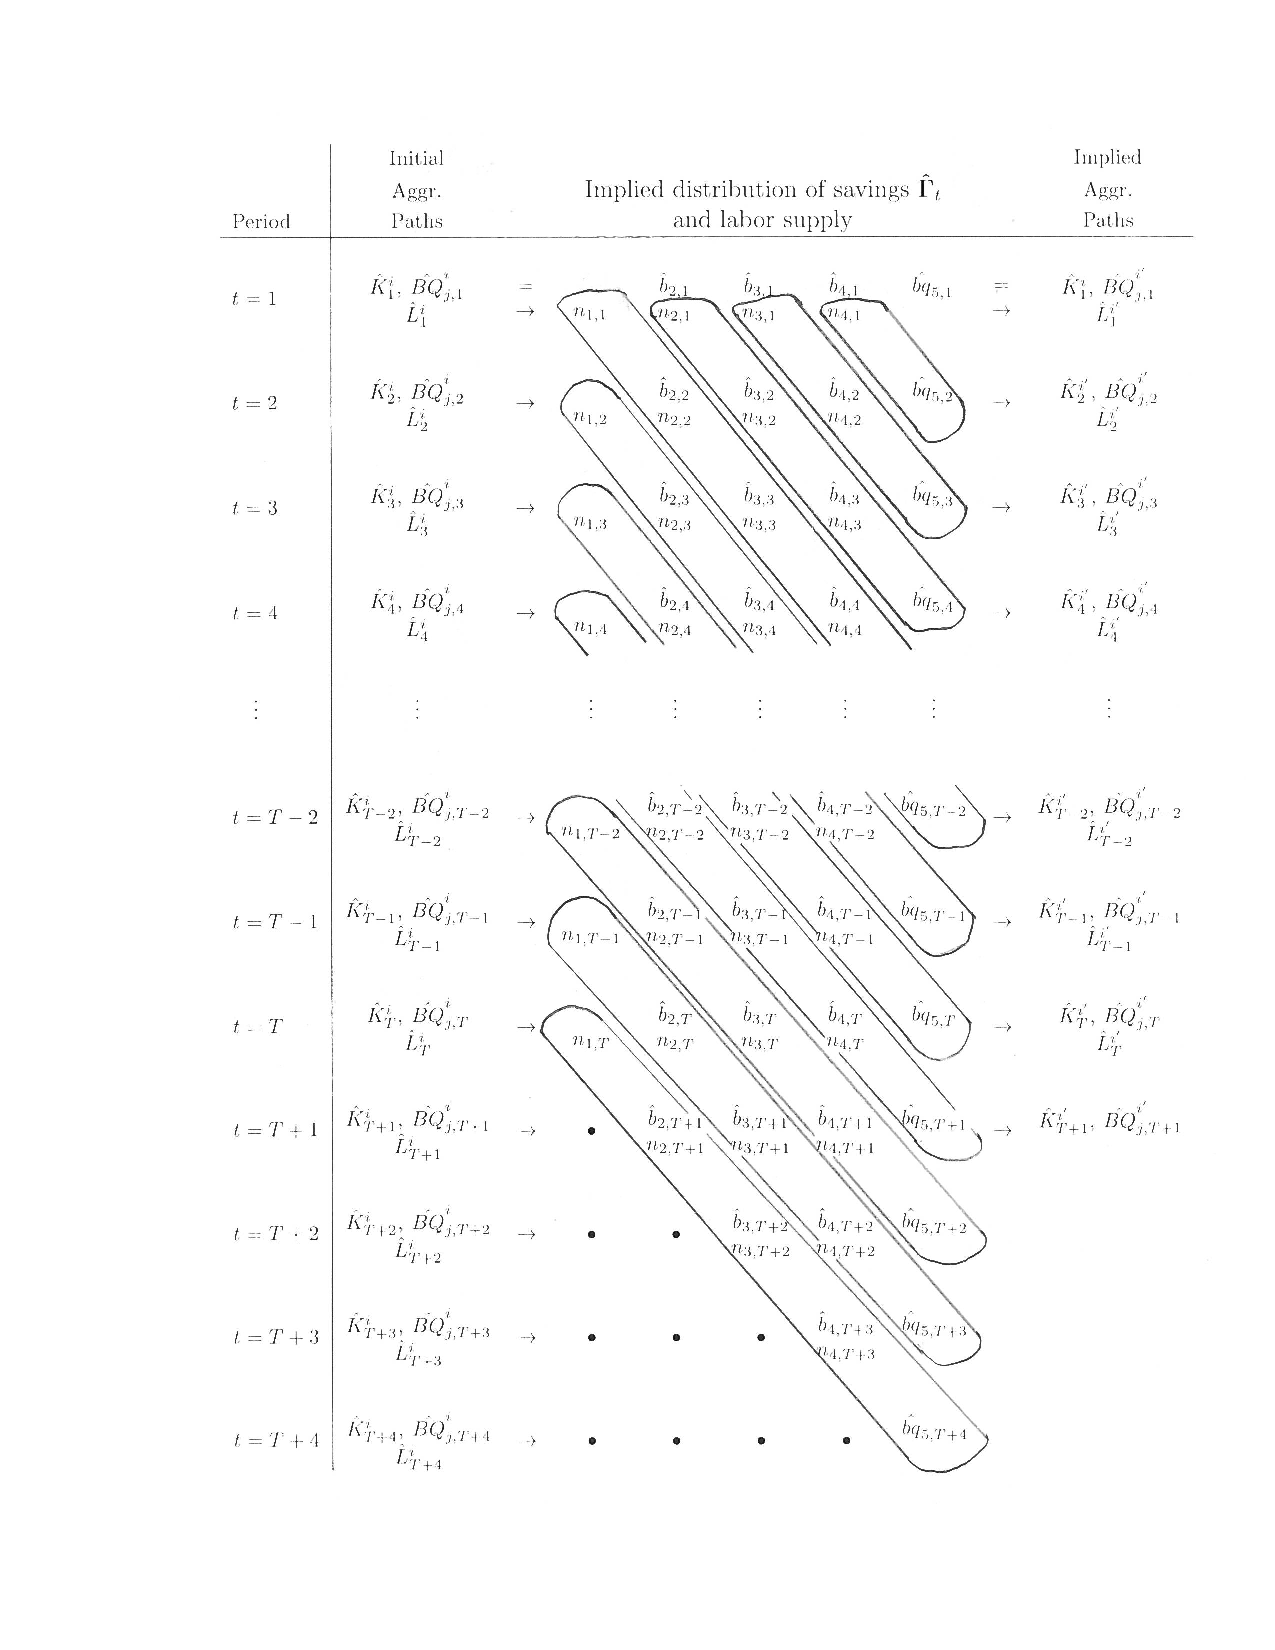
\includegraphics{images/TPIdiag.pdf}}}
  \end{figure}


  % THIS IS THE CODE FOR THE TABLE UNDERLYING THE FIGURE ABOVE
  % \begin{tabular}{>{\footnotesize}l| >{\footnotesize}c >{\footnotesize}c >{\footnotesize}c >{\footnotesize}c >{\footnotesize}c >{\footnotesize}c >{\footnotesize}c >{\footnotesize}c >{\footnotesize}c}
  %          & Initial & & & & & & & & Implied \\
  %          & Aggr. & & \multicolumn{5}{c}{Implied distribution of savings $\bm{\hat{\Gamma}}_t$} & & Aggr. \\
  %   Period & Paths    & & \multicolumn{5}{c}{and labor supply}   & & Paths    \\
  %   \hline
  %   & & & & & & & & & \\
  %   $t=1$ & $\begin{matrix}\hat{K}_1^i, \: \hat{BQ}_{j,1}^i \\ \hat{L}_1^i\end{matrix}$ & $\begin{matrix}= \\ \rightarrow\end{matrix}$ & $\begin{matrix}\: \\ n_{1,1}\end{matrix}$ & $\begin{matrix}\hat{b}_{2,1} \\ n_{2,1}\end{matrix}$ & $\begin{matrix}\hat{b}_{3,1} \\ n_{3,1}\end{matrix}$ & $\begin{matrix}\hat{b}_{4,1} \\ n_{4,1}\end{matrix}$ & $\begin{matrix}\hat{bq}_{5,1} \\ \,\end{matrix}$ & $\begin{matrix}= \\ \rightarrow\end{matrix}$ & $\begin{matrix}\hat{K}_1^i, \: \hat{BQ}_{j,1}^{i'} \\ \hat{L}^{i'}_1\end{matrix}$ \\[10mm]
  %   $t=2$ & $\begin{matrix}\hat{K}_2^i, \: \hat{BQ}_{j,2}^i \\ \hat{L}^i_2\end{matrix}$ & $\rightarrow$ & $\begin{matrix}\: \\ n_{1,2}\end{matrix}$ & $\begin{matrix}\hat{b}_{2,2} \\ n_{2,2}\end{matrix}$ & $\begin{matrix}\hat{b}_{3,2} \\ n_{3,2}\end{matrix}$ & $\begin{matrix}\hat{b}_{4,2} \\ n_{4,2}\end{matrix}$ & $\begin{matrix}\hat{bq}_{5,2} \\ \,\end{matrix}$ & $\rightarrow$ & $\begin{matrix}\hat{K}_2^{i'}, \: \hat{BQ}_{j,2}^{i'} \\ \hat{L}^{i'}_2\end{matrix}$ \\[10mm]
  %   $t=3$ & $\begin{matrix}\hat{K}_3^i, \: \hat{BQ}_{j,3}^i \\ \hat{L}^i_3\end{matrix}$ & $\rightarrow$ & $\begin{matrix}\: \\ n_{1,3}\end{matrix}$ & $\begin{matrix}\hat{b}_{2,3} \\ n_{2,3}\end{matrix}$ & $\begin{matrix}\hat{b}_{3,3} \\ n_{3,3}\end{matrix}$ & $\begin{matrix}\hat{b}_{4,3} \\ n_{4,3}\end{matrix}$ & $\begin{matrix}\hat{bq}_{5,3} \\ \,\end{matrix}$ & $\rightarrow$ & $\begin{matrix}\hat{K}_3^{i'}, \: \hat{BQ}_{j,3}^{i'} \\ \hat{L}^{i'}_3\end{matrix}$ \\[10mm]
  %   $t=4$ & $\begin{matrix}\hat{K}_4^i, \: \hat{BQ}_{j,4}^i \\ \hat{L}^i_4\end{matrix}$ & $\rightarrow$ & $\begin{matrix}\: \\ n_{1,4}\end{matrix}$ & $\begin{matrix}\hat{b}_{2,4} \\ n_{2,4}\end{matrix}$ & $\begin{matrix}\hat{b}_{3,4} \\ n_{3,4}\end{matrix}$ & $\begin{matrix}\hat{b}_{4,4} \\ n_{4,4}\end{matrix}$ & $\begin{matrix}\hat{bq}_{5,4} \\ \,\end{matrix}$ & $\rightarrow$ & $\begin{matrix}\hat{K}_4^{i'}, \: \hat{BQ}_{j,4}^{i'} \\ \hat{L}^{i'}_4\end{matrix}$ \\[10mm]
  %   $\quad\vdots$ & $\vdots$ & & $\vdots$ & $\vdots$ & $\vdots$ & $\vdots$ & $\vdots$ & & $\vdots$ \\[10mm]
  %   $t=T-2$ & $\begin{matrix}\hat{K}_{T-2}^i, \: \hat{BQ}_{j,T-2}^i \\ \hat{L}^i_{T-2}\end{matrix}$ & $\rightarrow$ & $\begin{matrix}\: \\ n_{1,T-2}\end{matrix}$ & $\begin{matrix}\hat{b}_{2,T-2} \\ n_{2,T-2}\end{matrix}$ & $\begin{matrix}\hat{b}_{3,T-2} \\ n_{3,T-2}\end{matrix}$ & $\begin{matrix}\hat{b}_{4,T-2} \\ n_{4,T-2}\end{matrix}$ & $\begin{matrix}\hat{bq}_{5,T-2} \\ \,\end{matrix}$ & $\rightarrow$ & $\begin{matrix}\hat{K}_{T-2}^{i'}, \: \hat{BQ}_{j,T-2}^{i'} \\ \hat{L}^{i'}_{T-2}\end{matrix}$ \\[10mm]
  %   $t=T-1$ & $\begin{matrix}\hat{K}_{T-1}^i, \: \hat{BQ}_{j,T-1}^i \\ \hat{L}^i_{T-1}\end{matrix}$ & $\rightarrow$ & $\begin{matrix}\: \\ n_{1,T-1}\end{matrix}$ & $\begin{matrix}\hat{b}_{2,T-1} \\ n_{2,T-1}\end{matrix}$ & $\begin{matrix}\hat{b}_{3,T-1} \\ n_{3,T-1}\end{matrix}$ & $\begin{matrix}\hat{b}_{4,T-1} \\ n_{4,T-1}\end{matrix}$ & $\begin{matrix}\hat{bq}_{5,T-1} \\ \,\end{matrix}$ & $\rightarrow$ & $\begin{matrix}\hat{K}_{T-1}^{i'}, \: \hat{BQ}_{j,T-1}^{i'} \\ \hat{L}^{i'}_{T-1}\end{matrix}$ \\[10mm]
  %   $t=T$ & $\begin{matrix}\hat{K}_{T}^i, \: \hat{BQ}_{j,T}^i \\ \hat{L}^i_{T}\end{matrix}$ & $\rightarrow$ & $\begin{matrix}\: \\ n_{1,T}\end{matrix}$ & $\begin{matrix}\hat{b}_{2,T} \\ n_{2,T}\end{matrix}$ & $\begin{matrix}\hat{b}_{3,T} \\ n_{3,T}\end{matrix}$ & $\begin{matrix}\hat{b}_{4,T} \\ n_{4,T}\end{matrix}$ & $\begin{matrix}\hat{bq}_{5,T} \\ \,\end{matrix}$ & $\rightarrow$ & $\begin{matrix}\hat{K}_{T}^{i'}, \: \hat{BQ}_{j,T}^{i'} \\ \hat{L}^{i'}_{T}\end{matrix}$ \\[10mm]
  %   $t=T+1$ & $\begin{matrix}\hat{K}_{T+1}^i, \: \hat{BQ}_{j,T+1}^i \\ \hat{L}^i_{T+1}\end{matrix}$ & $\rightarrow$ & $\bullet$ & $\begin{matrix}\hat{b}_{2,T+1} \\ n_{2,T+1}\end{matrix}$ & $\begin{matrix}\hat{b}_{3,T+1} \\ n_{3,T+1}\end{matrix}$ & $\begin{matrix}\hat{b}_{4,T+1} \\ n_{4,T+1}\end{matrix}$ & $\begin{matrix}\hat{bq}_{5,T+1} \\ \,\end{matrix}$ & $\rightarrow$ & $\begin{matrix}\hat{K}_{T+1}^{i'}, \: \hat{BQ}_{j,T+1}^{i'} \\ \:\end{matrix}$ \\[10mm]
  %   $t=T+2$ & $\begin{matrix}\hat{K}_{T+2}^i, \: \hat{BQ}_{j,T+2}^i \\ \hat{L}^i_{T+2}\end{matrix}$ & $\rightarrow$ & $\bullet$ & $\bullet$ & $\begin{matrix}\hat{b}_{3,T+2} \\ n_{3,T+2}\end{matrix}$ & $\begin{matrix}\hat{b}_{4,T+2} \\ n_{4,T+2}\end{matrix}$ & $\begin{matrix}\hat{bq}_{5,T+2} \\ \,\end{matrix}$ & & \\[10mm]
  %   $t=T+3$ & $\begin{matrix}\hat{K}_{T+3}^i, \: \hat{BQ}_{j,T+3}^i \\ \hat{L}^i_{T+3}\end{matrix}$ & $\rightarrow$ & $\bullet$ & $\bullet$ & $\bullet$ & $\begin{matrix}\hat{b}_{4,T+3} \\ n_{4,T+3}\end{matrix}$ & $\begin{matrix}\hat{bq}_{5,T+3} \\ \,\end{matrix}$ & & \\[10mm]
  %   $t=T+4$ & $\begin{matrix}\hat{K}_{T+4}^i, \: \hat{BQ}_{j,T+4}^i \\ \hat{L}^i_{T+4}\end{matrix}$ & $\rightarrow$ & $\bullet$ & $\bullet$ & $\bullet$ & $\bullet$ & $\begin{matrix}\hat{bq}_{5,T+4} \\ \,\end{matrix}$ & & \\
  % \end{tabular}
  % \clearpage

  Once the set of lifetime saving and labor supply decisions has been computed for all individuals alive in $1\leq t\leq T$, we use the household decisions to compute a new implied time path of the aggregate capital stock and aggregate labor. The implied paths of the aggregate capital stock $\bm{\hat{K}}^{i'}=\{\hat{K}_1^i,\hat{K}_2^{i'},...\hat{K}_T^{i'}\}$, aggregate labor $\bm{\hat{L}}^{i'}=\{\hat{L}_1^i,\hat{L}_2^{i'},...\hat{L}_T^{i'}\}$, and total bequests received $\bm{\hat{BQ}}_j^{i'}=\{\hat{BQ}_{j,1}^i,\hat{BQ}_{j,2}^{i'},...\hat{BQ}_{j,T}^{i'}\}$ in general do not equal the initial guessed paths $\bm{\hat{K}}^{i}=\{\hat{K}_1^i,\hat{K}_2^{i},...\hat{K}_T^{i}\}$, $\bm{\hat{L}}^{i}=\{\hat{L}_1^i,\hat{L}_2^{i},...\hat{L}_T^{i}\}$, and $\bm{\hat{BQ}}_j^{i}=\{\hat{BQ}_{j,1}^i,\hat{BQ}_{j,2}^{i},...\hat{BQ}_{j,T}^{i}\}$ used to compute the household savings and labor supply decisions $\bm{\hat{K}}^{i'}\neq\bm{\hat{K}}^i$, $\bm{\hat{L}}^{i'}\neq\bm{\hat{L}}^i$, and $\bm{\hat{BQ}}_j^{i'}\neq\bm{\hat{BQ}}_j^i$.

  Let $\norm{\:\cdot\:}$ be a norm on the space of time paths of the aggregate capital stock $\bm{\hat{K}}\in\mathcal{K}\subset\mathbb{R}_{++}^T$, aggregate labor supply $\bm{\hat{L}}\in\mathcal{L}\subset\mathbb{R}_{++}^T$, and $J$ paths of total bequests received $\bm{\hat{BQ}}_j\in\mathcal{B}\subset\mathbb{R}_{++}^T$. Then the fixed point necessary for the equilibrium transition path from Definition \ref{DefEquilNonSS} has been found when the distance between these $J+2$ paths is arbitrarily close to zero.
  \begin{equation}\label{EqTPIconverge}
    \norm{\Bigl[\bm{\hat{K}}^{i'}, \bm{\hat{L}}^{i'},\bigl\{\bm{\hat{BQ}}_j^{i'}\bigr\}_{j=1}^J\Bigr] - \Bigl[\bm{\hat{K}}^{i},\bm{\hat{L}}^{i},\bigl\{\bm{\hat{BQ}}_j^{i}\bigr\}_{j=1}^J\Bigr]} \leq \ve \quad\text{for}\quad \ve>0
  \end{equation}
  If the fixed point has not been found $\norm{\Bigl[\bm{\hat{K}}^{i'}, \bm{\hat{L}}^{i'},\bigl\{\bm{\hat{BQ}}_j^{i'}\bigr\}_{j=1}^J\Bigr] - \Bigl[\bm{\hat{K}}^{i},\bm{\hat{L}}^{i},\bigl\{\bm{\hat{BQ}}_j^{i}\bigr\}_{j=1}^J\Bigr]} > \ve$, then new transition paths for the aggregate capital stock and aggregate labor are generated as a convex combination of $\Bigl[\bm{\hat{K}}^{i'},\bm{\hat{L}}^{i'},\bigl\{\bm{\hat{BQ}}_j^{i'}\bigr\}_{j=1}^J\Bigr]$ and $\Bigl[\bm{\hat{K}}^{i},\bm{\hat{L}}^{i},\bigl\{\bm{\hat{BQ}}_j^{i}\bigr\}_{j=1}^J\Bigr]$.
  \begin{equation}\label{EqTPInewpath}
    \begin{split}
      \bm{\hat{K}}^{i+1} &= \nu\bm{\hat{K}}^{i'} + (1-\nu)\bm{\hat{K}}^{i} \\
      \bm{\hat{L}}^{i+1} &= \nu\bm{\hat{L}}^{i'} + (1-\nu)\bm{\hat{L}}^{i} \\
      \bm{\hat{BQ}}_1^{i+1} &= \nu\bm{\hat{BQ}}_1^{i'} + (1-\nu)\bm{\hat{BQ}}_1^{i} \\
      &\vdots \\
      \bm{\hat{BQ}}_J^{i+1} &= \nu\bm{\hat{BQ}}_J^{i'} + (1-\nu)\bm{\hat{BQ}}_J^{i}
    \end{split} \quad\quad\text{for}\quad \nu\in(0,1]
  \end{equation}
  This process is repeated until the initial transition paths for the aggregate capital stock, aggregate labor, and total bequests received are consistent with the transition paths implied by those beliefs and household and firm optimization.

  In essence, the TPI method iterates on individual beliefs about the time path of prices represented by a time paths for the aggregate capital stock $\bm{\hat{K}}^i$, aggregate labor $\bm{\hat{L}}^i$, and total bequests received $\bm{\hat{BQ}}_j^i$ until a fixed point in beliefs is found that are consistent with the transition paths implied by optimization based on those beliefs.

  The following are the steps for computing a stationary non-steady-state equilibrium time path for the economy.
  \begin{enumerate}
    \item Input all initial parameters. See Table \ref{TabExogVars}.
      \begin{enumerate}
        \item The value for $T$ at which the non-steady-state transition path should have converged to the steady state should be at least as large as the number of periods it takes the population to reach its steady state $\bm{\bar{\omega}}$ as described in Appendix \ref{AppPopGrowth}.
      \end{enumerate}

    \item Choose an initial distribution of savings and intended bequests $\bm{\hat{\Gamma}}_1$ and then calculat the initial state of the stationarized aggregate capital stock $\hat{K}_1$ and total bequests received $\hat{BQ}_{j,1}$ consistent with $\bm{\hat{\Gamma}}_1$ according to \eqref{EqMktClrCapStat} and \eqref{EqTotBeqStat1}.
      \begin{enumerate}
        \item Note that you must have the population weights from the previous period $\hat{\omega}_{s,0}$ and the growth rate between period 0 and period 1 $\tilde{g}_{n,1}$to calculate $\hat{BQ}_{j,1}$.
      \end{enumerate}
    \item Conjecture transition paths for the stationarized aggregate capital stock $\bm{\hat{K}}^1=\{\hat{K}^1_t\}_{t=1}^\infty$, stationarized aggregate labor $\bm{\hat{L}}^1=\{\hat{L}^1_t\}_{t=1}^\infty$, and total bequests received $\bm{\hat{BQ}}_j^1=\{\hat{BQ}^{1}_{j,t}\}_{t=1}^\infty$ where the only requirements are that $\hat{K}^i_1$ and $\hat{BQ}^i_{j,1}$ are functions of the initial distribution of savings $\bm{\hat{\Gamma}}_1$ for all $i$ is your initial state and that $\hat{K}^i_t=\bar{K}$, $\hat{L}^i_t=\bar{L}$, and $\hat{BQ}^i_{j,t}= \bar{BQ}_j$ for all $t\geq T$. The conjectured transition paths of the aggregate capital stock $\bm{\hat{K}}^i$ and aggregate labor $\bm{\hat{L}}^i$ imply specific transition paths for the real wage $\bm{\hat{w}}^i=\{\hat{w}^i_t\}_{t=1}^\infty$ and the real interest rate $\bm{r}^i=\{r^i_t\}_{t=1}^\infty$ through expressions \eqref{EqFOCwageStat} and \eqref{EqFOCrate}.
      \begin{enumerate}
        \item An intuitive choice for the time path of aggregate labor is the steady-state in every period $\hat{L}^1_t = \bar{L}$ for all $t$.
      \end{enumerate}
    \item With the conjectured transition paths $\bm{\hat{w}}^i$, $\bm{r}^i$, and $\bm{\hat{BQ}}_j^i$ one can solve for the lifetime policy functions of each household alive at time $1\leq t\leq T$ using the systems of Euler equations of the form \eqref{EqEulerLabStat}, \eqref{EqEulerSavStat}, and \eqref{EqEulerSavEpSstat} and following the diagram in Figure \ref{FigTPIdiag}.
    \item Use the implied distribution of savings and labor supply in each period (each row of $\hat{b}_{j,s,t}$ and $n_{j,s,t}$ in Figure \ref{FigTPIdiag}) to compute the new implied time paths for the aggregate capital stock $\bm{\hat{K}}^{i'} = \{\hat{K}_1^i,\hat{K}_2^{i'},...\hat{K}_T^{i'}\}$, aggregate labor supply $\bm{\hat{L}}^{i'} = \{\hat{L}_1^i,\hat{L}_2^{i'},...\hat{L}_T^{i'}\}$, and total bequests received $\bm{\hat{BQ}}_j^{i'} = \{\hat{BQ}_{j,1}^i,\hat{BQ}_{j,2}^{i'},...\hat{BQ}_{j,T}^{i'}\}$.
    \item Check the distance between the two sets time paths.
      \begin{equation*}
        \norm{\Bigl[\bm{\hat{K}}^{i'}, \bm{\hat{L}}^{i'},\bigl\{\bm{\hat{BQ}}_j^{i'}\bigr\}_{j=1}^J\Bigr] - \Bigl[\bm{\hat{K}}^{i},\bm{\hat{L}}^{i},\bigl\{\bm{\hat{BQ}}_j^{i}\bigr\}_{j=1}^J\Bigr]}
      \end{equation*}
      \begin{enumerate}
        \item If the distance between the initial time paths and the implied time paths is less-than-or-equal-to some convergence criterion $\ve>0$, then the fixed point has been achieved and the equilibrium time path has been found \eqref{EqTPIconverge}.
        \item If the distance between the initial time paths and the implied time paths is greater than some convergence criterion $\norm{\cdot}>\ve$, then update the guess for the time paths according to \eqref{EqTPInewpath} and repeat steps (4) through (6) until a fixed point is reached.
      \end{enumerate}
  \end{enumerate}








\chapter{Miscellaneous}
\index{Miscellaneous%
@\emph{Miscellaneous}}%



\section{Incorporating Feedbacks with Micro Tax Simulations}\label{SecMicro}

  Follow this algorthim:
  \begin{itemize}
    \item Period 1
    \begin{itemize}
      \item Use current IRS public use sample.
      \item Run the following within-period routine
      \begin{itemize}
        \item Do the static tax analysis of this sample, save the results
        \item Summarize the public use sample by aggregating into bins over age and earnings ability
        \item Use this as a starting point for the dynamic macro model
        \item Get values for fundamental interest rates and effective wages for next period
      \end{itemize}
    \end{itemize}
  \item Period 2
    \begin{itemize}
      \item “Age” the public use data demographically by one year.
      \item Let wages and interest rates rise by the amounts predicted in the macro model.
      \item Rerun the within-period routine
    \end{itemize}
  \item Iterate over periods until end of forecast period is reached.
  \end{itemize}

\section{Calibration}
  \subsection{Tax Bend Points}
      We use IRS data which summarizes individual tax returns for 2011 by 19 income categories and 4 filing statuses.  For each filing status we fit the mapping from reported income into adjusted gross income (AGI) using a sufficiently high-order polynomial.  We then use this function to solve for the income level which corresponds to each of the five bend points in the tax code for each filing type.
      \begin{table}[ht]
        \caption{AGI and Income Bend Points}
        \label{Calib_Bend_Tab1}
        \centering
        AGI Bend Points
        \begin{tabular}{|r|r|r|r|r|} \hline 
          Tax rate & Married Joint & Married Separate & Head of Household & Single \\ \hline 
          10\% & 17,400 & 8700 & 12,400 & 8700 \\ \hline 
          15\% & 70,700 & 35,350 & 47,350 & 35,350 \\ \hline 
          25\% & 142,700 & 71,350 & 122,300 & 85,650 \\ \hline 
          28\% & 217,450 & 108,725 & 198,050 & 178,650 \\ \hline 
          33\% & 388,350 & 194,175 & 388,350 & 388,350 \\ \hline 
        \end{tabular}
        \\
        Corresponding Reported Income Bendpoints
        \begin{tabular}{|r|r|r|r|r|} \hline 
          Tax rate & Married Joint & Married Separate & Head of Household & Single \\ \hline 
          0\%  & 5850  & 91 & 756 & 1435 \\ \hline 
          10\% & 22,932 & 8591 & 12,911 & 9956 \\ \hline 
          15\% & 75,181 & 34,592 & 47,023 & 36,021 \\ \hline 
          25\% & 145,866 & 69,768 & 120,200 & 85,244 \\ \hline 
          28\% & 219,162 & 106,245 & 194,176 & 176,270 \\ \hline 
          33\% & 386,798 & 189,674 & 380,043 & 381,524 \\ \hline 
        \end{tabular}
      \end{table}

      We then fit a bivariate probabililty density function over income and filing type from the data.  For each bendpoint we calculate the probability density at that bendpoint and use these as weights in a weighted average over filing types to generate an aggregate bendpoint.
      \begin{table}[ht]
        \caption{Aggregated Bend Points}
        \label{Calib_Bend_Tab2}
        \centering
        \begin{tabular}{|r|r|} \hline 
          Tax rate & Bend Point \\ \hline 
          0\% & 2889 \\ \hline 
          10\% & 15,116 \\ \hline 
          15\% & 52,580 \\ \hline 
          25\% & 114,552 \\ \hline 
          28\% & 196,201 \\ \hline 
          33\% & 380,657 \\ \hline 
        \end{tabular}
      \end{table}

% Bibliography:
\clearpage
\bibliography{AEIBYUDyn_Bib}
\index{Bibliography@\emph{Bibliography}}%  

\printindex

\end{document}
